\clearpage
\phantomsection

\setcounter{chapter}{2}
\chapter[NHẬN DẠNG HỆ THỐNG SỬ DỤNG MẠNG HỌC SÂU]{Nhận dạng hệ thống sử dụng mạng học sâu}
\label{sec:ML}

% Trong chương này, tác giả đề xuất một kiến trúc mạng học sâu ISDNN sử dụng cho nhận dạng hệ thống viễn thông mMIMO. Đầu tiên, sơ lược về hai hướng tiếp cận sử dụng mạng nơ-ron sâu sẽ được giới thiệu. Kế đến là khái niệm về kỹ thuật mở rộng sâu (Deep unfolding). Một kiến trúc được mở rộng sâu từ bộ tối ưu MLE là DetNet được trình bày để so sánh ở mục các kết quả mô phỏng. Tiếp đến, từ một giải thuật ISD đã được đề xuất trong~\cite{Mandloi2017}, kết hợp với cách tiếp cận mở rộng sâu tại~\cite{Liao2020}, một mạng nơ-ron sâu tên ISDNN được đề xuất để nhận dạng hệ thống. Kiến trúc mạng ISDNN được đề xuất cho cả hai mô hình kênh truyền có cấu trúc và không sử dụng cấu trúc đã được trình bày tại chương~\ref{sec:CRB}. Các bước mô phỏng và đánh giá sẽ được đưa ra để cho thấy tiềm năng của phương pháp đề xuất và kết luận của chương. 

% \section{Giới thiệu về mạng nơ-ron sâu và mở rộng sâu}
% \begin{figure} [H]
%     \centering
%     \begin{tikzpicture}[x=2.2cm,y=1.4cm]
%         \node[antenna, thick, scale=0.6] at (5mm, 14mm) (Rx0) {};
%         \node at (5mm, 30mm) (text_Rx0) {Rx $1$};
%         \draw[line] (5mm, 14mm) -- (18mm,14mm);
    
%         \node[antenna, thick, scale=0.6] at (0mm, 0mm) (Rx1) {};
%         \node at (0mm, 16mm) (text_Rx0) {Rx $2$};
%         \draw[line] (0mm, 0) -- (18mm, 0);

%         \node[antenna, thick, scale=0.6] at (-5mm, -14mm) (Rx2) {};
%         \node at (-5mm, 2mm) (text_Rx0) {Rx $3$};
%         \draw[line] (-5mm, -14mm) -- (18mm, -14mm);
    
%         \node[scale=1.5] at (0mm, -23mm) (dotss) {$\mathbf{\vdots}$};
    
%         \node[antenna, thick, scale=0.6] at (-10mm, -35mm) (RxL) {};
%         \node at (-10mm, -19mm) (text_RxL) {Rx $L$};
%         \draw[line] (-10mm, -35mm) -- (18mm, -35mm);

    
%       \readlist\Nnod{4,5,5,5,3} % array of number of nodes per layer
%       \readlist\Nstr{L,m,m,m,T} % array of string number of nodes per layer
%       \readlist\Cstr{\strut x,a^{\prev},a^{\prev},a^{\prev}, s} % array of coefficient symbol per layer
%       \def\yshift{0.5} % shift last node for dots
      
%       \foreachitem \N \in \Nnod{ % loop over layers
%         \def\lay{\Ncnt} % alias of index of current layer
%         \pgfmathsetmacro\prev{int(\Ncnt-1)} % number of previous layer
%         \message{\lay,}
%         \foreach \i [evaluate={\c=int(\i==\N); \y=\N/2-\i-\c*\yshift;
%                      \index=(\i<\N?int(\i):"\Nstr[\lay]");
%                      \x=\lay; \n=\nstyle;}] in {1,...,\N}{ % loop over nodes
%           % NODES
%           \node[node \n] (N\lay-\i) at (\x,\y) {$\Cstr[\lay]_{\index}$};
          
%           % CONNECTIONS
%           \ifnum\lay>1 % connect to previous layer
%             \foreach \j in {1,...,\Nnod[\prev]}{ % loop over nodes in previous layer
%               \draw[connect,white,line width=1.2] (N\prev-\j) -- (N\lay-\i);
%               \draw[connect] (N\prev-\j) -- (N\lay-\i);
%               %\draw[connect] (N\prev-\j.0) -- (N\lay-\i.180); % connect to left
%             }
%           \fi % else: nothing to connect first layer
          
%         }
%         \path (N\lay-\N) --++ (0,1+\yshift) node[midway,scale=1.5] {$\vdots$};
%       }
      
%       % LABELS
%       \node[above=2,align=center,green!60!black] at (1, 0) {Đầu vào};
%       \node[above=2,align=center,blue!60!black] at (65mm, 0) {Lớp ẩn};
%       \node[above=2,align=center,red!60!black] at (110mm, 0) {Đầu ra};
      
%     \end{tikzpicture}
%     \caption{Minh họa sử dụng DNN để nhận dạng hệ thống viễn thông.}
%     \label{fig:DNN_model}
% \end{figure}
% Trong chương~\ref{sec:back}, các phương pháp nhận dạng hệ thống sử dụng các phương pháp ML/DL được chia làm ba loại, trong đó phương pháp sử dụng các mạng nơ-ron đang được quan tâm nghiên cứu. Các mạng nơ-ron sâu được sử dụng rộng rãi trong các ứng dụng như xử lý tiếng nói, ngôn ngữ tự nhiên, hình ảnh, thị giác máy, trò chơi trực tuyến~\cite{Samek2021}. Mười năm trở lại đây, đã có nhiều nghiên cứu ứng dụng các mạng DNN khác nhau cho vấn đề nhận dạng hệ thống viễn thông không dây. Hình~\ref{fig:DNN_model} biểu diễn mô hình minh họa việc sử dụng DNN để ước lượng kênh truyền và khôi phục tín hiệu gốc. Có thể chia các phương pháp này thành hai hướng tiếp cận, bao gồm hướng dữ liệu (data-driven) và hướng mô hình (model-driven)~\cite{Liao2020}. Các phương pháp data-driven trực tiếp học các đặc trưng từ một tập lớn các dữ liệu (dataset) để phục vụ cho các mục đích như ước lượng kênh truyền, phản hồi CSI,~\ldots Tuy các phương pháp data-driven đều cho độ chính xác cao nhưng vẫn có những thách thức khi yêu cầu số lượng mẫu rất lớn và kéo theo đó là thời gian/chi phí cho việc đào tạo lớn. Các phương pháp model-driven~\cite{He2019} có thể khắc phục một phần các hạn chế này bằng việc tối ưu/đưa thêm các tham số học vào các kiến trúc có sẵn để kết hợp ưu điểm của data-driven và các mô hình toán học truyền thống. 

% Gần đây, kỹ thuật mở rộng sâu~\cite{Wisdom2016} là một giải pháp tiềm năng để chuyển các giải thuật truyền thống thành các kiến trúc mạng DNN theo hướng tiếp cận model-driven. Chi tiết về mở rộng sâu được trình bày tại~\cite{John2014}, các phương pháp yêu cầu các vòng lặp đi lặp lại (iteractive inference) có thể dễ dàng chuyển đổi sang các lớp của một mạng NN. Sau đó, sử dụng các giải thuật giảm dần độ dốc (GD - Gradient Descent) để đào tạo tham số trên các lớp mạng. Sau $K$ lớp đào tạo tương tự như $K$ vòng lặp trong thuật toán gốc, mô hình có thể đạt được mục tiêu mong muốn. Ví dụ, DetNet~\cite{Samuel2017} là một mạng DNN dựa trên việc mở rộng sâu bộ nhận dạng MLE và sử dụng giảm dần độ dốc dự kiến (PGD - Projected Gradient Descent)~\cite{Chen2015}. Trong mục tiếp theo, mạng nơ-ron sâu DetNet sẽ được giới thiệu ngắn gọn và kết quả của DetNet sẽ được so sánh với kiến trúc mạng đề xuất.

\section{Mạng nơ-ron sâu DetNet}

Vẫn sử dụng mô hình hệ thống mMIMO đã trình bày ở phần~\ref{sec:mMIMO}.
\begin{equation}
    \mathbf{x} = \mathbf{H} \mathbf{s} + \mathbf{w}
\end{equation}
Các phần tử trong ma trận kênh truyền $\mathbf{H}$ được biểu diễn dưới dạng số phức, đại diện cho cả ảnh hưởng về biên độ và pha gây ra bởi kênh. Cách biểu diễn này phù hợp trên lý thuyết, các phương pháp giải tối ưu, và các phần mềm mô phỏng như Matlab. Tuy nhiên, trong học máy/học sâu, các giá trị số phức thường được tách riêng thành phần thực ($\Re$) và phần ảo ($\Im$) như sau:
% riêng biệt.
% Quá trình học của thành phần thực và ảo thuộc một giá trị số phức cũng được tách riêng biệt, qua đó phát huy lợi thế của ML/DL.
% Bên cạnh đó, các phép toán phổ biến trong xử lý tín hiệu như chuyển vị, liên hợp phức cũng sẽ được thực hiện dễ dàng hơn nếu tách riêng thành phần thực và ảo.
% Từ các lý do trên, các phương pháp sử dụng ML/DL nhận dạng kênh sẽ chuyển đổi tất cả các giá trị phức sang dạng thực trước khi đưa vào quá trình đào tạo trong mạng. Các mạng ML/DL này thường được phát triển trên ngôn ngữ Python và các thư viện nền tảng thông dụng như Tensorflow\footnote{\url{https://github.com/tensorflow/tensorflow}} của Google hay Pytorch\footnote{\url{https://github.com/pytorch/pytorch}} của Facebook. 
% % Do vậy, không làm mất đi tính tổng quát, trong chương này, 
% Các ma trận và véc-tơ trên mô hình kênh kể trên sẽ được biểu diễn dưới dạng các thành phần thực ($\Re$) và phần ảo ($\Im$) như sau:
\begin{equation}
\label{eq:matrixtras1}
    \mathbf{s}=\left[\begin{array}{l}
    \Re(\mathbf{s}) \\
    \Im(\mathbf{s})
    \end{array}\right] ;
    \mathbf{x}=\left[\begin{array}{l}
    \Re(\mathbf{x}) \\
    \Im(\mathbf{x})
    \end{array}\right] ; 
    \mathbf{w}=\left[\begin{array}{l}
    \Re(\mathbf{w}) \\
    \Im(\mathbf{w})
    \end{array}\right]
\end{equation}

\begin{equation}
\label{eq:matrixtras2}
    \mathbf{H}=\left[\begin{array}{cc}
    \Re(\mathbf{H}) & -\Im(\mathbf{H}) \\
    \Im(\mathbf{H}) & \Re(\mathbf{H})
    \end{array}\right]
\end{equation}
trong đó, $\mathbf{H} \in \mathbb{R}^{2L \times 2T}$, $\mathbf{s} \in \mathbb{R}^{2T \times 1}$, $\mathbf{w} \in \mathbb{R}^{2L \times 1}$, và $\mathbf{x} \in \mathbb{R}^{2L \times 1}$. Thông thường, các kiến trúc mạng ML/DL sử dụng để ước lượng kênh truyền giả sử rằng ma trận kênh truyền $\mathbf{H}$ được mô hình hoá dưới dạng không sử dụng cấu trúc, hay các hệ số của $\mathbf{H}$ được chọn ngẫu nhiên và không bị ảnh hưởng bởi các thông số vật lý khác như DoA, cấu hình mảng ăng-ten,~\ldots Để tìm bộ nhận dạng cho hệ thống kể trên, định nghĩa hàm mất mát $\mathcal{L}\left(\mathbf{s} ; \hat{\mathbf{s}}_{\boldsymbol{\Theta}}(\mathbf{H}, \mathbf{x})\right)$ là khoảng cách giữa véc-tơ ký hiệu gốc và véc-tơ ký hiệu được ước lượng. Tìm giá trị $\boldsymbol{\Theta}$ bằng cách tối thiểu hoá hàm mất mát kể trên như sau:
\begin{equation}
\label{eq:lossf}
\min _{\boldsymbol{\Theta}} \mathbb{E}\left\{\mathcal{L}\left(\mathbf{s} ; \hat{\mathbf{s}}_{\boldsymbol{\Theta}}(\mathbf{H}, \mathbf{x})\right)\right\}
\end{equation}

Sử dụng giải thuật MLE để giải~(\ref{eq:lossf}) được:
\begin{equation}
\label{eq:mle}
\hat{\mathbf{s}}_{\boldsymbol{\Theta}}(\mathbf{H}, \mathbf{x})=\arg \min _{\mathbf{s} \in \mathbb{R}^{2T}}\|\mathbf{x}-\mathbf{H} \mathbf{s}\|^2
\end{equation}
% Tuy nhiên, độ phức tạp của MLE sẽ tăng theo cấp số mũ $\mathcal{O}(2^T)$ nên khó để triển khai trong các hệ mMIMO. Do vậy, DetNet được đề xuất nhằm tạo ra một kiến trúc mạng DNN tiệm cận độ chính xác với MLE. Trong nghiên cứu gốc, thay vì tạo ra một mạng nơ-ron nhằm ánh xạ trực tiếp từ $\mathbf{x}$ về $\mathbf{s}$, việc phân tách $\mathbf{x}$ thành các thành phần $\mathbf{H}, \mathbf{s},$ và $\mathbf{w}$ như~(\ref{eq:3.6}) sẽ cho hiệu quả cao hơn.
% \begin{equation}
%     \label{eq:3.6}
%     \mathbf{H}^\top \mathbf{x}=\mathbf{H}^\top \mathbf{H s}+\mathbf{H}^\top \mathbf{w}
% \end{equation}

DetNet dựa trên phương pháp PGD thực hiện việc tối ưu MLE như phương trình~(\ref{eq:mle}).
% Đạo hàm riêng được tách như trên (\ref{eq:pgd}) sử dụng luật chuỗi (chain rule).
% \begin{equation}
% \label{eq:pgd}
%     \begin{aligned}
%     \hat{\mathbf{s}}_{k+1} & =\boldsymbol{\Gamma}\left[\hat{\mathbf{s}}_k-\left.\delta_k \frac{\partial\|\mathbf{x}-\mathbf{H} \mathbf{s}\|^2}{\partial \mathbf{s}}\right|_{\mathbf{s}=\hat{\mathbf{s}}_k}\right] \\
%     & = \boldsymbol{\Gamma}\left[\hat{\mathbf{s}}_k-\delta_k \mathbf{H}^\top \mathbf{x}+\delta_k \mathbf{H}^\top \mathbf{H} \hat{\mathbf{s}}_k\right]
%     \end{aligned}
% \end{equation}
% với $\hat{\mathbf{s}}_k$ là véc-tơ giá trị nguồn ước lượng tại lớp thứ $k$, $\boldsymbol{\Gamma}[.]$ là một phép biến đổi phi tuyến tính, và $\delta_k$ là độ dài bước của quá trình học. 
Kiến trúc của một lớp mạng DetNet được biểu diễn dưới dạng ma trận là:
\allowdisplaybreaks
\begin{subequations}
\begin{alignat}{4}
    \mathbf{z}_k & =\rho\left(\mathbf{W}^1_{k}\left[\begin{array}{c}
    \mathbf{H}^\top \mathbf{x} \\
    \hat{\mathbf{s}}_k \\
    \mathbf{H}^\top \mathbf{H} \hat{\mathbf{s}}_k \\
    \mathbf{v}_k
    \end{array}\right]+\mathbf{b}^1_{k}\right) \\
    \hat{\mathbf{s}}_{k+1} & =\psi_{t_k}\left(\mathbf{W}^2_{k} \mathbf{z}_k+ \mathbf{b}^2_{k}\right) \\
    {\mathbf{v}}_{k+1} & =\mathbf{W}^3_{k} \mathbf{z}_k+ 
    \mathbf{b}^3_{k} \\
    \hat{\mathbf{s}}_1 & =\mathbf{0}_{2T}
\end{alignat}
\end{subequations}
trong đó, $k = 1, \ldots, K$ là số các lớp của mạng DetNet, $\rho$ là một toán tử tuyến tính. $\psi_{t_k}$ ký hiệu cho phép biến đổi phi tuyến tính phân đoạn, ở các mức $t$ khác nhau, $\psi_{t_k}(s)$ có biểu diễn toán học như sau:
\begin{equation}
    \psi_{t_k}(s)=-1+\frac{\rho\left(s + t_k \right)}{\left|t_k\right|}-\frac{\rho\left(s- t_k \right)}{\left|t_k\right|}
\end{equation}

% \begin{figure}[tb]
%     \centering
%     \begin{tikzpicture}
%         \node (B11) [field6, fill=red!10!white] at (0, 0) {$\mathbf{H}^\top \mathbf{x}$};
%         \node (B21) [below=10mm of B11, field6, fill=red!10!white] {$\mathbf{v}_k$};
%         \node (B31) [below=10mm of B21, field6, fill=red!10!white] {$\hat{\mathbf{s}}_k$};
%         \node (B41) [below=10mm of B31, field6, fill=red!10!white] {$\mathbf{H}^\top \mathbf{H}$};

        
%         \node (B32) [right=10mm of B31.south east, anchor=north, circle, fill=blue!10!white, draw=black] {$\times$}; 
%         \node (B22) [right=25mm of B21, circle, fill=blue!10!white, draw=black] {$\operatorname{con}$};
%         \node (B33) [below=11mm of B22, circle, fill=blue!10!white, draw=black] {$\times$};
%         \node (B34) [below=4mm of B33, field8, fill=green!10!white, draw=black] {$\mathbf{W}^1_{k}$};
%         \node (B35) [right=7mm of B33, circle, fill=blue!10!white, draw=black] {$+$};
%         \node (B36) [below=4mm of B35, field8, fill=green!10!white, draw=black] {$\mathbf{b}^1_{k}$};

%         \node (B37) [circle, fill=blue!10!white, draw=black] at (70mm, -30mm) {$\rho$};
%         \node (B38) [right=40mm of B33, circle, fill=blue!10!white, draw=black] {$\times$};
%         \node (B39) [below=4mm of B38, field8, fill=green!10!white, draw=black] {$\mathbf{W}^2_{k}$};
%         \node (B310) [right=7mm of B38, circle, fill=blue!10!white, draw=black] {$+$};
%         \node (B311) [below=4mm of B310, field8, fill=green!10!white, draw=black] {$\mathbf{b}^2_{k}$};
%         \node (B312) [right=7mm of B310, circle, fill=blue!10!white, draw=black] {$\Psi$};

%         \node (B23) [above=24.2mm of B39, circle, fill=blue!10!white, draw=black] {$\times$};
%         \node (B24) [right=7mm of B23, circle, fill=blue!10!white, draw=black] {$+$};
%         \node (B25) [above=4mm of B23, field8, fill=green!10!white, draw=black] {$\mathbf{W}^3_{k}$};
%         \node (B26) [above=4mm of B24, field8, fill=green!10!white, draw=black] {$\mathbf{b}^3_{k}$};

%         \node (Bvk1) [right=123mm of B21, field6, fill=red!10!white] {$\mathbf{v}_{k+1}$};
%         \node (Bxk1) [right=123mm of B31, field6, fill=red!10!white] {$\hat{\mathbf{s}}_{k+1}$};

%         \draw[arrow] (B312) -- (Bxk1);
%         \draw[arrow] (B24) -- (Bvk1);
%         \draw[arrow] (B310) -- (B312);
%         \draw[arrow] (B38) -- (B310);
%         \draw[arrow] (B23) -- (B24);
%         \draw[arrow] (B25) -- (B23);
%         \draw[arrow] (B26) -- (B24);
%         \draw[arrow] (B311) -- (B310);
%         \draw[arrow] (B39) -- (B38);
%         \draw[arrow] (B33) -- (B35);
%         \draw[arrow] (B36) -- (B35);
%         \draw[arrow] (B34) -- (B33);
%         \draw[arrow] (B22) -- (B33);

%         \draw[arrow] (B21) -- (B22);
%         \draw[line] (B11) -- ([yshift=-3mm]B11.south);
%         \draw[arrow] ([yshift=-3mm]B11.south) -| (B22);
%         \draw[line] (B31) -- ([xshift=3mm]B31.east);
%         \draw[arrow] ([xshift=3mm]B31.east) |- ([yshift=-1.5mm]B22.west);
%         \draw[line] (B32) -- ([xshift=3mm]B32.east);
%         \draw[arrow] ([xshift=3mm]B32.east) |- ([yshift=-3mm]B22.west);

%         \draw[arrow] (B31) |- ([yshift=3mm]B32);
%         \draw[arrow] (B41) |- ([yshift=-3mm]B32);

%         \draw[arrow] (B37) |- (B38);
%         \draw[arrow] (B37) |- (B23);
%         \draw[arrow] (B35) |- (B37);
        
%         \draw[arrow] (B41) -- (150mm, -60mm);
%         \draw[arrow] (Bvk1) -- (150mm, -20mm);
%         \draw[arrow] (Bxk1) -- (150mm, -41mm);
%         \draw[arrow] (B11) -- (150mm, 0mm);

%         % Legends
%         \node[rectangle, draw=black, dashed, fill=black!5!white, minimum width=140mm, minimum height=35mm] at (70mm, -85mm) {};

%         \node (B51) [field6, fill=red!10!white] at (22mm, -78mm) {Giá trị \\đầu vào/đầu ra};

%         \node (B61) [below=4mm of B51, field8, fill=green!10!white, draw=black] {Giá trị học};

%         \node (B52) [right=7mm of B51, circle, fill=blue!10!white, draw=black] {$\times$};
%         \draw[arrow] (B52) -- ([xshift=3mm]B52.east) node [pos=0, right=3mm] {Nhân};

%         \node (B53) [below=7mm of B52, circle, fill=blue!10!white, draw=black] {$+$};
%         \draw[arrow] (B53) -- ([xshift=3mm]B53.east) node [pos=0, right=3mm] {Cộng};

%         \node (B54) [right=20mm of B52, circle, fill=blue!10!white, draw=black] {$\rho$};
%         \draw[arrow] (B54) -- ([xshift=10mm]B54.east) node [pos=0, right=10mm, above, label={below}:{tuyến tính}] {Toán tử};

%         \node (B55) [right=20mm of B53, circle, fill=blue!10!white, draw=black] {$\Psi$};
%         \draw[arrow] (B55) -- ([xshift=10mm]B55.east) node [pos=0, right=11mm, above, label={below}:{phi tuyến tính}] {Toán tử};

%         \node (B56) [right=28mm of B54, circle, fill=blue!10!white, draw=black] {$\operatorname{con}$};
%         \draw[arrow] (B56) -- ([xshift=10mm]B56.east) node [pos=0, right=11mm, above, label={below}:{véc-tơ}] {Nối};
         
%     \end{tikzpicture}
%     \caption{Kiến trúc của một lớp trong kiến trúc mạng DetNet~\cite{Samuel2017}.}
%     \label{fig:detnet}
% \end{figure}

% \begin{figure}[ht]
%     \centering
%     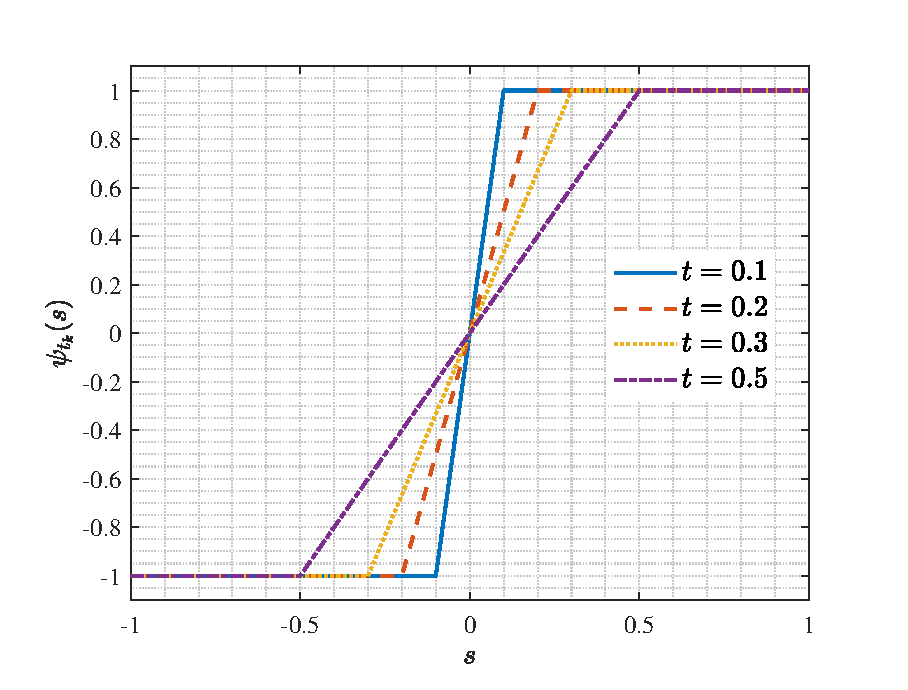
\includegraphics[width=.8\linewidth]{figures/soft_sign.eps}
%     \caption{Hàm phi tuyến tính phân đoạn $\psi_{t_k}(s)$ được sử dụng trong DetNet.}
%     \label{fig:soft_sign}
% \end{figure}
Các tham số của việc học sẽ bao gồm:
\begin{equation}
\boldsymbol{\Theta}=\left\{\mathbf{W}^1_{k}, \mathbf{b}^1_{k}, \mathbf{W}^2_{k}, \mathbf{b}^2_{k}, \mathbf{W}^3_{k}, \mathbf{b}^3_{ k}, t_k\right\}_{k=1}^K
\end{equation}

Sau mỗi vòng lặp (iteration), một hàm mất mát có dạng sai số bình phương trung bình (MSE - Mean Squared Error) sẽ tính toán sự sai khác của véc-tơ các ký hiệu ước lượng so với véc-tơ các ký hiệu gốc. Kết quả này được sử dụng để xem xét sự hội tụ của việc đào tạo, và được trả về cho giải thuật tối ưu (ví dụ: Adam) để tối ưu các tham số học của mạng. Hàm mất mát này được định nghĩa như dưới đây:
\begin{equation}
\label{eq:lossdetnet}
    \mathcal{L}(\mathbf{s} ; \hat{\mathbf{s}}_{\boldsymbol{\Theta}}(\mathbf{H}, \mathbf{x}))= \frac{1}{2T} \sum_{t=1}^{2T} {\left\| s_t-\hat{s}_t\right\|^2}
\end{equation}
% \begin{equation}
% \label{eq:lossdetnet}
%     l(\mathbf{s} ; \hat{\mathbf{s}}(\mathbf{H}, \mathbf{x}))=\sum_{k=1}^K \log (k) \frac{\left\|\mathbf{s}-\hat{\mathbf{s}}_k\right\|^2}{\|\mathbf{s}-\tilde{\mathbf{s}}\|^2}
% \end{equation}
% với $\tilde{\mathbf{s}}$ là ước lượng của $\mathbf{s}$ thu được từ bộ giải mã ZF như trình bày trong mục~\ref{sec:zf}. Lưu ý rằng, do $\mathbf{H}$ là ma trận của các số thực nên phép chuyển vị liên hợp phức $(.)^H$ sẽ được chuyển thành chuyển vị $(.)^\top$.
% \begin{equation}
%     \tilde{\mathbf{s}}=\left(\mathbf{H}^\top \mathbf{H}\right)^{-1} \mathbf{H}^\top \mathbf{x}
% \end{equation}

\section{Đề xuất mạng nơ-ron sâu ISDNN cho nhận dạng kênh truyền}
\subsection{Bộ nhận dạng ISD cho hệ thống mMIMO}

Bài báo đã đề xuất một bộ nhận dạng kênh truyền tuần tự lặp lại gọi tắt là ISD để đạt được hiệu suất của MMSE với độ phức tạp thấp.
\begin{equation}
    \hat{\mathbf{s}}_{MMSE}=\left(\mathbf{H}^\top \mathbf{H}+\frac{\sigma^2}{\mathbb{E}(\mathbf{s})} \mathbf{I}_{2T}\right)^{-1} \mathbf{H}^\top \mathbf{x}=\mathbf{P}^{-1} \mathbf{q}
\end{equation}
ký hiệu $\mathbf{G}_\mathbf{H} = \mathbf{H}^\top \mathbf{H}$, $\mathbf{P} = \mathbf{H}^\top \mathbf{H}+\frac{\sigma^2}{\mathbb{E}(\mathbf{s})} \mathbf{I}_{2T}$, và $\mathbf{q} = \mathbf{H}^\top \mathbf{x}$. 
Các thành phần đường chéo của ma trận $\mathbf{P}$ tạo thành ma trận đường chéo $\mathbf{D} = \operatorname{diag}(\mathbf{P})$.
% Định nghĩa ma trận $\mathbf{P}$ tạo thành ma trận $\mathbf{D} = \operatorname{diag}(\mathbf{H}^\top \mathbf{H})$.
Lưu ý, độ phức tạp của việc nghịch đảo $\mathbf{P}$ là $\mathcal{O}(TL^3)$, sẽ tăng nhanh khi $L$ lớn. 

Để đạt được hiệu năng cao hơn với số lần lặp ít hơn, ISD đề xuất khởi tạo véc-tơ của các ký hiệu ước lượng ($\hat{\mathbf{s}}_1$) như trên phương trình~(\ref{eq:sinit}) thay vì đặt tất cả bằng $0$ như DetNet.
\begin{equation}
\label{eq:sinit}
    \hat{\mathbf{s}}_1=\mathbf{D}^{-1} \mathbf{q}=\left[s_1(1), s_1(2), \ldots, s_1(2T)\right]
\end{equation}

% Từ véc-tơ tín hiệu thu, tín hiệu của ăng-ten/người dùng thứ $j$ thu được bằng cách coi tín hiệu từ các ăng-ten/người dùng khác như tạp âm và loại bỏ chúng.
% \begin{equation}
%     \hat{\mathbf{x}}(j)=\mathbf{x}-\sum_{t=1, t \neq j}^{2T} \mathbf{h}_t \hat{s}_k(t)
% \end{equation}
% với $\hat{\mathbf{x}}(j)$ thu được, ký hiệu được gửi từ người dùng thứ $j$ được ước lượng như sau:
% \begin{equation}
% \label{eq:supdate}
%     \begin{aligned}
%         \hat{s}_{k+1}(j) & =\frac{\mathbf{h}_j^\top}{\left\|\mathbf{h}_j\right\|^2} \hat{\mathbf{x}}(j) \\ 
%         & = \hat{s}_k(j)+\frac{1}{\mathbf{G}_\mathbf{H}(j, j)}\left(\mathbf{q}(j)-\sum_{t=1}^{2T} \mathbf{G}_\mathbf{H}(j, t) s_k(t)\right)
%     \end{aligned}
% \end{equation}
% trong đó, $\mathbf{h}_j$ là cột thứ $j$ của ma trận $\mathbf{H}$, $\mathbf{G}_\mathbf{H}(i, j)$ là phần tử thứ $(i, j)$ của ma trận $\mathbf{G}_\mathbf{H}$, và $\mathbf{q}(j)$ là phần tử thứ $j$ của véc-tơ $\mathbf{q}$.
Véc-tơ các ký hiệu ước lượng $\hat{\mathbf{s}}$ được cập nhật như trong thuật toán~\ref{alg:cap} của giải thuật ISD. 
\begin{algorithm}[ht]
    \caption{Bộ nhận dạng Iterative Sequential.}\label{alg:cap}
    \hspace*{\algorithmicindent} \textbf{Input: $\mathbf{x}, \mathbf{H}, L, T, K, \sigma^2, \mathbb{E}(\mathbf{s})$} \\
    \hspace*{\algorithmicindent} \textbf{Output: $\hat{\mathbf{s}}_{out} = \hat{\mathbf{s}}^{2T}_K$} 
    \begin{algorithmic}[1]
        \State $\mathbf{G}_\mathbf{H} \leftarrow \mathbf{H}^\top \mathbf{H}$
        \State $\mathbf{P} \leftarrow \mathbf{G}_\mathbf{H} + \frac{\sigma^2}{\mathbb{E}(\mathbf{s})} \mathbf{I}_{2T}$
        \State $\mathbf{D} \leftarrow \operatorname{diag}(\mathbf{P})$
        \State $\mathbf{q} \leftarrow \mathbf{H}^\top \mathbf{x}$
        \State $\mathbf{s}_1 \leftarrow \mathbf{D}^{-1} \mathbf{q}$ \\
        \For{ $k=0, k < K$}
            \For{ $j=1, j \le 2T$}
                \State $\hat{s}_k(j+1) \leftarrow \hat{s}_k(j)+\frac{1}{\mathbf{G}_\mathbf{H}(j, j)}\left(\mathbf{q}(j)-\sum_{t=1}^{2T} \mathbf{G}_\mathbf{H}(j, t) \hat{s}_k(t)\right)$ \\ 
                \State $\hat{\mathbf{s}}_{k+1}^j \leftarrow\left[\hat{s}_{k+1}(1),~\ldots, \hat{s}_{k+1}(j), \hat{s}_k(j+1),~\ldots, \hat{s}_k(2T)\right]$
                \State $j \leftarrow j + 1$
            \EndFor
            \State $k \leftarrow k + 1$
        \EndFor
    \end{algorithmic}
\end{algorithm}

Để chứng minh giải thuật ISD là hiệu quả cho việc ước lượng kênh truyền, véc-tơ phần dư (sai số) sẽ được sử dụng. Cụ thể, véc-tơ phần dư thu được sau khi khởi tạo với các giá trị $\hat{\mathbf{s}}_1$ là:
\begin{equation}
    \mathbf{e}_1 = \mathbf{x} - \mathbf{H} \hat{\mathbf{s}}_1
\end{equation}
từ đó, véc-tơ phần dư sau khi cập nhật ký hiệu thứ $j$ tại lớp thứ $k$ sẽ được biểu diễn như sau:
\begin{equation}
    \mathbf{e}_k^{j}=\mathbf{x}-\mathbf{H} \hat{\mathbf{s}}_k^j
\end{equation}
thay $\hat{\mathbf{s}}_k^j$ bằng các biểu diễn hồi quy như trong giải thuật~\ref{alg:cap} thu được:
\begin{equation}
\label{eq:eupdate}
\begin{aligned}
    \mathbf{e}_k^{j} =\mathbf{e}_k^{j-1}-\mathbf{h}_{j} \frac{\mathbf{h}_j^\top}{\left\|\mathbf{h}_j\right\|^2} \mathbf{e}_k^{j-1}
    \end{aligned}
\end{equation}

Trong bài báo gốc, Mandloi M. và các cộng sự đã chứng minh rằng $\left\|\mathbf{e}_k^{j}\right\|^2<\left\|\mathbf{e}_k^{j-1}\right\|^2$. 
% Điều đó chỉ ra, mỗi khi ký hiệu thứ $j$ được cập nhật, véc-tơ phần dư sẽ được chiếu lên mặt phẳng `null' của cột thứ $j$ thuộc ma trận $\mathbf{H}$. Hay véc-tơ phần dư sẽ trực giao với $\mathbf{h}_j$, do đó $l_2-\operatorname{norm}$ bình phương của véc-tơ lỗi sẽ giảm sau mỗi lần ký hiệu $j$ được cập nhật cho đến khi véc-tơ $\mathbf{e}$ trực giao với không gian con kéo dài bởi cột của ma trận $\mathbf{H}$.

\subsection{Đề xuất mạng nơ-ron sâu ISDNN cho mô hình kênh truyền không sử dụng cấu trúc}
\label{sec:ISNN_nonstructured}

Từ giải thuật ISD được trình bày ở trên, theo hướng tiếp cận model-driven và kỹ thuật mở rộng sâu, một kiến trúc mạng nơ-ron sâu có tên ISDNN (Iterative Sequential Deep-neural Network) tương ứng cho mô hình kênh truyền không sử dụng cấu trúc (gọi tắt là \textbf{ISDNN không sử dụng cấu trúc}) được đề xuất. Đầu tiên, việc cập nhật các ký hiệu $\mathbf{s}$ tại dòng $9$ của giải thuật~\ref{alg:cap} được viết lại dưới dạng ma trận như sau:
\begin{equation}
\hat{\mathbf{s}}_{k+1}=\hat{\mathbf{s}}_k+\mathbf{e}_{k+1}
\end{equation}
trong đó, $\mathbf{e}_{k+1}$ là véc-tơ phần dư cũng được viết dưới dạng ma trận là:
\begin{equation}
    \mathbf{e}_{k+1}=\mathbf{D}^{-1}\left(\mathbf{H}^\top \mathbf{x}-\mathbf{H}^\top \mathbf{H} \hat{\mathbf{s}}_k\right)
\end{equation}
với ma trận đường chéo $\mathbf{D}$ được đơn giản hoá lấy ý tưởng từ bộ nhận dạng ZF khi không có thông tin về SNR tại bên thu, tức nghịch đảo của ma trận Gram ($\mathbf{G}_\mathbf{H}$), $\mathbf{D}~=~\operatorname{diag}(\mathbf{H}^\top \mathbf{H})$. 
% Việc thay đổi này làm giảm độ phức tạp của phép nghịch đảo $\mathbf{D}$. 
Nhận thấy rằng, $\hat{\mathbf{s}}_{k+1}$ không chỉ chịu ảnh hưởng trực tiếp bởi $\mathbf{e}_{k+1}$ mà còn tất cả các véc-tơ phần dư trước đó $\mathbf{e}_{k}, \mathbf{e}_{k-1},~\ldots, \mathbf{e}_{1}$ như biểu diễn ở công thức~(\ref{eq:eupdate}). Do vậy, để đạt được hiệu quả cao hơn trong việc loại bỏ tạp âm từ các người dùng khác, các tham số học được thêm vào $\alpha^1$ vào mỗi lớp (layer) của mạng nơ-ron.
\begin{equation}
\label{eq:supdate1}
\hat{\mathbf{s}}_{k+1}=\hat{\mathbf{s}}_k+\mathbf{e}_{k+1}+\alpha_k^{1} \mathbf{e}_k+\alpha_{k-1}^{1} \mathbf{e}_{k-1}+\cdots+\alpha_1^{1} \mathbf{e}_1
\end{equation}

Tuy nhiên, do mối tương quan giữa các véc-tơ phần dư liền kề là lớn nhất, nên trong mạng ISDNN chỉ xem xét ảnh hưởng của $\mathbf{e}_k$ ở lớp thứ $k$ nhằm đơn giản hoá kiến trúc mạng. Phương trình~(\ref{eq:supdate1}) trở thành:
\begin{equation}
\boldsymbol{\mu}_{k}=\hat{\mathbf{s}}_k+\mathbf{e}_{k+1}+\alpha_k^1 \mathbf{e}_k
\end{equation}

Thay vì gán trực tiếp $\hat{\mathbf{s}}_{k+1} = \boldsymbol{\mu}_k$, sự tương quan giữa $\boldsymbol{\mu}_k$ và $\hat{\mathbf{s}}_k$ được xem xét trước khi đưa làm đầu vào của lớp tiếp theo. Sử dụng kết hợp lồi (convex combination) của $\hat{\mathbf{s}}_k$ và $\boldsymbol{\mu}_k$ với hệ số $\alpha^2$. Do đó, $\hat{\mathbf{s}}_{k+1}$ chịu ảnh hưởng bởi cả $\hat{\mathbf{s}}_k$ và $\boldsymbol{\mu}_k$ theo tỷ lệ $\alpha^2$. 
Trong đó, $\alpha^2_k$ là tham số có thể học, $\sum_{i=k}^{k+1} \alpha_i^{2} \hat{\mathbf{s}}_i$ với $\sum_{i=k}^{k+1} \alpha_i^{2}=1$, tại mỗi lớp. Kết hợp tuyến tính của $\hat{\mathbf{s}}_k$ và $\boldsymbol{\mu}_k$ có dạng như sau:
\begin{equation}
\hat{\mathbf{s}}_{k+1}=\left(1-\alpha_k^2\right) \boldsymbol{\mu}_k + \alpha_k^2 \hat{\mathbf{s}}_k
\end{equation}

Ngoài ra, để đạt được độ chính xác cao hơn ở các loại điều chế bậc cao như (16-QAM, 64-QAM,~\ldots), véc-tơ phần dư sẽ được điều chỉnh linh hoạt hơn bằng cách thêm hai bộ biến đổi tuyến tính vào kiến trúc mạng ISDNN để cập nhật $\mathbf{e}_k$ trước khi nhân với $\alpha^1_k$.
\begin{equation}
\mathbf{e}_k \leftarrow w^2_{k}\left(w^1_{k} \mathbf{e}_k+b^1_{k}\right)+b^2_{k}
\end{equation}

Bộ nhận dạng trong các các nghiên cứu trước đây tuần tự đưa các dữ liệu huấn luyện chỉ ứng với một lần tạo dữ liệu độc lập qua mạng, tức $\mathbf{H} \in \mathbb{R}^{2L \times 2T}$, $\mathbf{s} \in \mathbb{R}^{2T \times 1}$, và $\mathbf{x} \in \mathbb{R}^{2L \times 1}$. Điều này làm giảm đáng kể tốc độ học của một mạng DNN do không tận dụng được lợi thế của kiểu dữ liệu ten-sơ (tensor), cho phép thao tác với các biến đa chiều. Do đó, điểm cải tiến tiếp theo của kiến trúc mạng ISDNN đó là sử dụng `Batch~size' lớn hơn rất nhiều. Với `\textit{bs}' (Batch~size) là lượng dữ liệu được sử dụng trong một vòng lặp. Các dữ liệu đầu vào của mạng ISDNN sẽ được chuyển sang dạng ten-sơ $3$ chiều như sau:
\begin{subequations}
    \begin{align}
        \mathbf{E}_k &\leftarrow [\mathbf{e}_k^1, \mathbf{e}_k^2,~\ldots, \mathbf{e}_k^{bs}]\\
        \hat{\mathbf{S}}_k &\leftarrow [\hat{\mathbf{s}}_k^1, \hat{\mathbf{s}}_k^2,~\ldots, \hat{\mathbf{s}}_k^{bs}] \\
        \mathbf{X}_k &\leftarrow [\mathbf{x}_k^1, \mathbf{x}_k^2,~\ldots, \mathbf{x}_k^{bs}] \\
        \mathbf{H}   &\leftarrow [\mathbf{H}^1, \mathbf{H}^2,~\ldots, \mathbf{H}^{bs}]  
    \end{align}
\end{subequations}

Các phép toán biến đổi ten-sơ, ví dụ, phép nhân các ma trận được chuyển đổi thành nhân các ten-sơ $3$~chiều được thực hiện bằng hàm `\textit{torch.bmm}'\footnote{\url{https://pytorch.org/docs/stable/generated/torch.bmm.html}} của thư viện nền tảng Pytorch. Tuy nhiên, do đây là đề xuất về mặt kỹ thuật lập trình nên trong các phần tiếp theo, các ký hiệu toán học vẫn được giữ ở dạng nhân ma trận tương tự như $bs = 1$ để tránh sự nhầm lẫn.

Kiến trúc cuối cùng của mạng ISDNN cho mô hình kênh truyền không sử dụng cấu trúc được đề xuất trong luận văn như trên hình~\ref{fig:ISD}. 
% So với giải thuật ISD được đề xuất trước đó, mạng nơ-ron sâu ISDNN được đề xuất có sự cải tiến như sau: (i) thêm véc-tơ phần dư của lớp trước đó và tham số học $\alpha^1$ để ước lượng $\hat{\mathbf{s}}$; (ii) tham số học $\alpha^2$ được thêm vào để tăng tính chính xác của việc học; (iii) véc-tơ phần dư được đưa qua hai bộ biến đổi để có được tính linh hoạt cho các loại điều chế bậc cao; (iv) sử dụng Batch size lớn để giảm thời gian học.
\begin{figure}[ht]
    \centering
    \begin{tikzpicture}
        \node (B11) [field6, fill=red!10!white] at (0, 0) {$\mathbf{e}_k$};
        \node (B21) [below=10mm of B11, field6, fill=red!10!white] {$\hat{\mathbf{s}}_k$};
        \node (B31) [below=10mm of B21, field6, fill=red!10!white] {$\mathbf{H}^\top \mathbf{H}$};
        \node (B41) [below=10mm of B31, field6, fill=red!10!white] {$\mathbf{H}^\top \mathbf{x}$};
        \node (B51) [below=10mm of B41, field6, fill=red!10!white] {$\mathbf{D}^{-1}$};

        \node (B12) [right=5mm of B11, circle, fill=blue!10!white, draw=black] {$\times$};
        \node (B13) [right=5mm of B12, circle, fill=blue!10!white, draw=black] {$+$};
        \node (B14) [right=5mm of B13, circle, fill=blue!10!white, draw=black] {$\times$};
        \node (B15) [right=5mm of B14, circle, fill=blue!10!white, draw=black] {$+$};
        \node (B16) [right=5mm of B15, circle, fill=blue!10!white, draw=black] {$\times$};
        \node (B17) [right=18mm of B16, field8, fill=green!10!white, draw=black] {$\alpha^2_k$};
        \node (B18) [right=5mm of B17, circle, fill=blue!10!white, draw=black] {$\times$};

        \node (B61) [below=4mm of B12, field8, fill=green!10!white, draw=black] {$w^1_{k}$};
        \node (B62) [below=4mm of B13, field8, fill=green!10!white, draw=black] {$b^1_{k}$};
        \node (B63) [below=4mm of B14, field8, fill=green!10!white, draw=black] {$w^2_{k}$};
        \node (B64) [below=4mm of B15, field8, fill=green!10!white, draw=black] {$b^2_{k}$};
        \node (B65) [below=4mm of B16, field8, fill=green!10!white, draw=black] {$\alpha^1_k$};

        \node (B22) [right=75mm of B21, circle, fill=blue!10!white, draw=black] {$+$};
        \node (B23) [below=12mm of B18, circle, fill=blue!10!white, draw=black] {$+$};
        \node (B24) [right=3mm of B23, circle, fill=blue!10!white, draw=black] {$\Psi$};

        \node (B25) [below=4mm of B23, circle, fill=blue!10!white, draw=black] {$\times$};
        \node (B26) [below=4mm of B25, field8, fill=green!10!white, draw=black] {$1 - \alpha^2_k$};

        \node (B32) [right=5mm of B31, circle, fill=blue!10!white, draw=black] {$\times$};
        \node (B42) [right=5mm of B41, circle, fill=blue!10!white, draw=black] {$-$};
        \node (B52) [right=5mm of B51, circle, fill=blue!10!white, draw=black] {$\times$};

        \node (Phi1) [right=123mm of B21, field6, fill=red!10!white] {$\hat{\mathbf{s}}_{k+1}$};
        \node (V1) [right=123mm of B51, field6, fill=red!10!white] {$\mathbf{e}_{k+1}$};

        \draw[arrow] (B11) -- (B12);
        \draw[arrow] (B12) -- (B13);
        \draw[arrow] (B13) -- (B14);
        \draw[arrow] (B14) -- (B15);
        \draw[arrow] (B15) -- (B16);
        \draw[arrow] (B17) -- (B18);
        
        \draw[arrow] (B61) -- (B12);
        \draw[arrow] (B62) -- (B13);
        \draw[arrow] (B63) -- (B14);
        \draw[arrow] (B64) -- (B15);
        \draw[arrow] (B65) -- (B16);

        \draw[arrow] (B21) -- (B22);
        \draw[arrow] (B31) -- (B32);
        \draw[arrow] (B41) -- (B42);
        \draw[arrow] (B51) -- (B52);
        \draw[arrow] (B52) -- (V1);

        \draw[arrow] (B18) -- (B23);
        \draw[arrow] (B23) -- (B24);
        \draw[arrow] (B24) -- (Phi1);

        \draw[arrow] (B16) -| (B22);
        \draw[arrow] (B25) -- (B23);
        \draw[arrow] (B26) -- (B25);
        \draw[line] (B22) -- ([xshift=3mm]B22.east);
        \draw[arrow] ([xshift=3mm]B22.east) |- (B25);
        \draw[line] (V1) -- ([yshift=15mm]V1.north);
        \draw[arrow] ([yshift=15mm]V1.north) -| (B22);

        \draw[arrow] (B21) -| (B32);
        \draw[arrow] (B32) -- (B42);
        \draw[arrow] (B42) -- (B52);

        \draw[line] (B21) -| ([xshift=-3mm, yshift=28mm]B21.west);
        \draw[arrow] ([xshift=-3mm, yshift=28mm]B21.west) -| (B18);

        \draw[arrow] (Phi1) -- ([xshift=3mm]Phi1.east);
        \draw[arrow] (V1) -- ([xshift=3mm]V1.east);

        % Legends
        \node[rectangle, draw=black, dashed, fill=black!5!white, minimum width=100mm, minimum height=35mm] at (70mm, -105mm) {};

        \node (B51) [field6, fill=red!10!white] at (37mm, -97mm) {Giá trị \\đầu vào/đầu ra};

        \node (B61) [below=4mm of B51, field8, fill=green!10!white, draw=black] {Giá trị học};

        \node (B52) [right=7mm of B51, circle, fill=blue!10!white, draw=black] {$\times$};
        \draw[arrow] (B52) -- ([xshift=3mm]B52.east) node [pos=0, right=3mm] {Nhân};

        \node (B53) [below=7mm of B52, circle, fill=blue!10!white, draw=black] {$+$};
        \draw[arrow] (B53) -- ([xshift=3mm]B53.east) node [pos=0, right=3mm] {Cộng};

        \node (B54) [right=20mm of B52, circle, fill=blue!10!white, draw=black] {$\Psi$};
        \draw[arrow] (B54) -- ([xshift=10mm]B54.east) node [pos=0, right=11mm, above, label={below}:{phi tuyến tính}] {Toán tử};

        \node (B55) [right=20mm of B53, circle, fill=blue!10!white, draw=black] {$-$};
        \draw[arrow] (B55) -- ([xshift=3mm]B55.east) node [pos=0, right=3mm] {Trừ};
    \end{tikzpicture}
    \caption{Kiến trúc của một lớp trong mạng nơ-ron sâu ISDNN đề xuất cho mô hình kênh truyền không sử dụng cấu trúc.}
    \label{fig:ISD}
\end{figure}
Các tham số khởi tạo của mạng ISDNN được đề xuất như sau để nhanh chóng đạt được sự hội tụ: $\hat{\mathbf{s}}_1 = \mathbf{D}^{-1}\mathbf{q}$; $\alpha^1_1$ được chọn ngẫu nhiên theo phân bố đều $\alpha^1_1~\in~\mathcal{U}[0 \;\; 1)$; $\alpha^2_1 = 0$,$5$; véc-tơ $\mathbf{e}_1$ được chọn lựa ngẫu nhiên theo phân bố đều $\mathbf{e}_1 \in  \mathcal{U}[0 \;\; 1)$. Do các đầu vào cho lớp tiếp theo $\hat{\mathbf{s}}_{k+1}$ cần được ánh xạ về khoảng giá trị $[-1.0 \;\; 1.0]$, một hàm kích hoạt (activation function) sẽ được sử dụng. Trong DL, có nhiều hàm kích hoạt được sử dụng rộng rãi như ReLu, Tanh, Sigmoid,~\ldots Cụ thể, mạng ISDNN lựa chọn sử dụng hàm Tanh có biểu diễn toán học như sau:
\begin{equation}
    \Psi(s) = \operatorname{Tanh}(s) = \frac{e^s - e^{-s}}{e^s + e^{-s}}
\end{equation}
% \begin{figure}[ht]
%     \centering
%     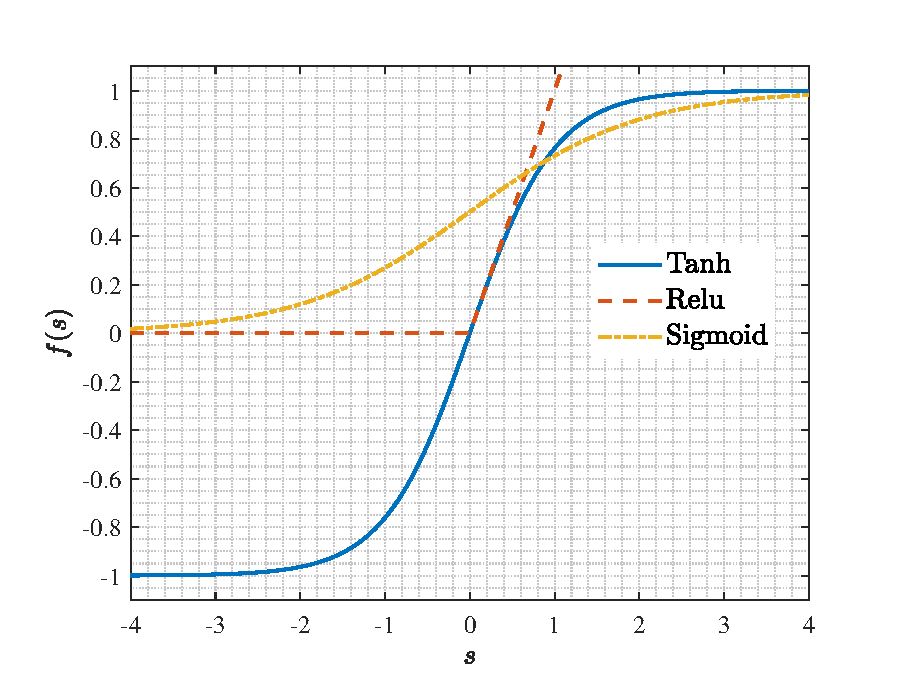
\includegraphics[width=.8\linewidth]{figures/tanh.eps}
%     \caption{Minh họa một số hàm kích hoạt được dùng trong kiến trúc đề xuất.}
%     \label{fig:tanh}
% \end{figure}

Các tham số của việc học sẽ bao gồm:
\begin{equation}
\boldsymbol{\Theta}=\left\{w^1_{k}, b^1_{k}, w^2_{k}, b^2_{k}, \alpha^1_k, \alpha^2_k \right\}_{k=1}^K
\end{equation}

Một hàm mất mát MSE cũng được định nghĩa như trên phương trình~(\ref{eq:lossdetnet}) của DetNet để biểu diễn sự hội tụ của mạng học sâu ISDNN và bước back-propagate của một mạng NN.

Bốn bước của một vòng lặp trong quá trình học như sau:
\begin{enumerate}
    \item Khởi tạo các tham số ban đầu và véc-tơ phần dư của mạng ISDNN: $\mathbf{s}_1, \mathbf{e}_1$, $\alpha^1_1, \alpha^2_1$.

    \item Bộ dữ liệu được đưa qua $K$ lớp của mạng (forward propagation), sau đó ước lượng sự mất mát qua hàm $\mathcal{L}(\mathbf{s}; \hat{\mathbf{s}}_{\boldsymbol{\Theta}}(\mathbf{H}, \mathbf{x}))$.

    \item Back-propagate $\mathcal{L}(\mathbf{s}; \hat{\mathbf{s}}_{\boldsymbol{\Theta}}(\mathbf{H}, \mathbf{x}))$ để thu được độ dốc (gradient).

    \item Từ gradient thu được, sử dụng một thuật toán tối ưu, ví dụ là Adam, cập nhật các tham số học $\boldsymbol{\Theta}=\left\{w^1_{k}, b^1_{k}, w^2_{k}, b^2_{k}, \alpha^1_k, \alpha^2_k \right\}_{k=1}^K$.
\end{enumerate}

\subsection{Đề xuất mạng nơ-ron sâu ISDNN cho mô hình kênh truyền có cấu trúc}

Khi mô hình kênh truyền dạng có cấu trúc như đã trình bày tại chương~\ref{sec:CRB}, một phần thông tin bên lề gồm DoA và cấu hình mảng ăng-ten tại bên thu được đề xuất sử dụng cho việc học của mạng ISDNN. Lý do chọn thông tin DoA là do trong các hệ mMIMO, kỹ thuật định hướng búp sóng (beamforming) có vai trò đặc biệt quan trọng trong việc tăng công suất truyền và giảm tỷ lệ tạp âm liên người dùng. Trước khi kỹ thuật beamforming có thể được sử dụng, việc biết hướng cần phát, hay hướng của người dùng (UE - User Equipment) là điều kiện cần có. Góc phát này được ước lượng thông qua tín hiệu từ các phiên truyền đường lên trước đó. Các thuật toán phổ biến được sử dụng để ước lượng hướng sóng đến như phương pháp CBF, Capon, hay MUSIC. 
\begin{equation}
    \label{eq:28}
    h_{l, t} = \beta_{l, t} e^{\varphi_{l, t}} = \beta_{l, t} e^{-i k_s c_l (\theta_{l, t}, \phi_{l, t})}
\end{equation}

Với giả thiết rằng DoA, tức các véc-tơ $\boldsymbol\theta, \boldsymbol\phi$, của các UE đã được trạm cơ sở ước lượng và khả dụng trước khi thực hiện ước lượng kênh truyền, kiến trúc ISDNN sẽ được sửa đổi để phù hợp hơn với mô hình kênh có cấu trúc như trong phương trình~(\ref{eq:28}) (gọi tắt là \textbf{ISDNN có cấu trúc}). Trước hết, thay vì phải ước lượng ma trận $\mathbf{H}$, do biết trước $\boldsymbol\theta, \boldsymbol\phi$ cũng như cấu hình của mảng ăng-ten tại trạm cơ sở, ma trận $\mathbf{H}$ được giản ước về chỉ còn thành phần hệ số khuếch đại phức của các tia ($\hat{\boldsymbol{\beta}}$). Phương trình~(\ref{eq:betahat}) biểu diễn các hệ số của ma trận kênh truyền trong trường hợp đơn giản, chỉ có tầm nhìn thẳng (LOS) hay $M = 1$.
\begin{equation}
\label{eq:betahat}
    \hat{\beta}_{l, t} = \frac{h_{l, t}} {\varphi_{l,t}}= \frac{h_{l, t}}{e^{-i k_s c_l (\theta_{l,t}, \phi_{l, t})}}
\end{equation}
Dùng phép chia vô hướng ở đây là do giả thiết các hệ số trong mô hình kênh truyền trên (\ref{eq:28}) là dạng rời rạc và vô hướng. Thực hiện tương tự với véc-tơ tín hiệu thu được $\mathbf{x}$. Giả thiết rằng, với toàn bộ thông tin véc-tơ lái $\boldsymbol{\varphi}$, véc-tơ $\mathbf{x}$ có thể được biến đổi về dạng $\hat{\mathbf{x}}$ khi kênh truyền chỉ được đại diện bởi các hệ số $\boldsymbol{\beta}$ như trên phương trình~(\ref{eq:betahat}) thông qua phép biến đổi $f_1$.
\begin{equation}
    \hat{\mathbf{x}} \longleftarrow f_1(\mathbf{x}, \boldsymbol{\varphi})
\end{equation}

Từ ma trận $\hat{\boldsymbol{\beta}}$ và véc-tơ $\hat{\mathbf{x}}$ thu được, các dữ liệu đầu vào còn lại trong mạng ISDNN cũng được thay đổi thông qua một tập các hàm xử lý tín hiệu đơn giản gọi tắt là $f_2$. Trong đó, hai giá trị $\mathbf{D}$ và $\hat{\mathbf{s}}_{1}$ có biểu diễn là:
\begin{equation}
    \begin{aligned}
        \mathbf{D} &= \operatorname{diag}(\hat{\boldsymbol{\beta}}^\top \hat{\boldsymbol{\beta}}) \\
        \hat{\mathbf{s}}_{1} &= \mathbf{D}^{-1} \hat{\boldsymbol{\beta}}^\top \hat{\mathbf{x}}
    \end{aligned}
\end{equation}

Kiến trúc một lớp mạng ISDNN cho kênh truyền có cấu trúc với thông tin bên lề là DoA tại bên thu được biểu diễn như trên hình~\ref{fig:ISD_structured}. Các tham số khởi tạo và quá trình đào tạo của mạng vẫn tương tự như kiến trúc ISDNN đã được trình bày sử dụng cho mô hình kênh truyền không sử dụng cấu trúc tại mục~\ref{sec:ISNN_nonstructured}.
\begin{figure}[ht]
    \centering
    \begin{tikzpicture}
        \node (B11) [field6, fill=red!10!white] at (0, 0) {$\mathbf{e}_k$};
        \node (B21) [below=10mm of B11, field6, fill=red!10!white] {$\hat{\mathbf{s}}_k$};

        \node (B12) [right=5mm of B11, circle, fill=blue!10!white, draw=black] {$\times$};
        \node (B13) [right=5mm of B12, circle, fill=blue!10!white, draw=black] {$+$};
        \node (B14) [right=5mm of B13, circle, fill=blue!10!white, draw=black] {$\times$};
        \node (B15) [right=5mm of B14, circle, fill=blue!10!white, draw=black] {$+$};
        \node (B16) [right=5mm of B15, circle, fill=blue!10!white, draw=black] {$\times$};
        \node (B17) [right=18mm of B16, field8, fill=green!10!white, draw=black] {$\alpha^2_k$};
        \node (B18) [right=5mm of B17, circle, fill=blue!10!white, draw=black] {$\times$};

        \node (B61) [below=4mm of B12, field8, fill=green!10!white, draw=black] {$w^1_{k}$};
        \node (B62) [below=4mm of B13, field8, fill=green!10!white, draw=black] {$b^1_{k}$};
        \node (B63) [below=4mm of B14, field8, fill=green!10!white, draw=black] {$w^2_{k}$};
        \node (B64) [below=4mm of B15, field8, fill=green!10!white, draw=black] {$b^2_{k}$};
        \node (B65) [below=4mm of B16, field8, fill=green!10!white, draw=black] {$\alpha^1_k$};

        \node (B31) [below=14mm of B64, field6, fill=red!10!white] {$\hat{\boldsymbol{\beta}}^\top \hat{\boldsymbol{\beta}}$};
        \node (B41) [below=10mm of B31, field6, fill=red!10!white] {$\hat{\boldsymbol{\beta}}^\top \hat{\mathbf{x}}$};
        \node (B51) [below=10mm of B41, field6, fill=red!10!white] {$\mathbf{D}^{-1}$};

        \node (B22) [right=75mm of B21, circle, fill=blue!10!white, draw=black] {$+$};
        \node (B23) [below=12mm of B18, circle, fill=blue!10!white, draw=black] {$+$};
        \node (B24) [right=3mm of B23, circle, fill=blue!10!white, draw=black] {$\Psi$};

        \node (B25) [below=4mm of B23, circle, fill=blue!10!white, draw=black] {$\times$};
        \node (B26) [below=4mm of B25, field8, fill=green!10!white, draw=black] {$1 - \alpha^2_k$};

        \node (B32) [right=5mm of B31, circle, fill=blue!10!white, draw=black] {$\times$};
        \node (B42) [right=5mm of B41, circle, fill=blue!10!white, draw=black] {$-$};
        \node (B52) [right=5mm of B51, circle, fill=blue!10!white, draw=black] {$\times$};

        \node (Phi1) [right=123mm of B21, field6, fill=red!10!white] {$\hat{\mathbf{s}}_{k+1}$};
        \node (V1) [right=66mm of B51, field6, fill=red!10!white] {$\mathbf{e}_{k+1}$};

        \node (H) [below=7mm of B21, field6, fill=red!10!white] {$\mathbf{H}$};
        \node (varphi) [below=10mm of H, field6, fill=red!10!white] {$\boldsymbol{\varphi}$};
        \node (x) [below=10mm of varphi, field6, fill=red!10!white] {$\mathbf{x}$};

        % \node (B71) [right=3mm of varphi, circle, fill=blue!10!white, draw=black] {$\times$};
        % \node (B72) [right=3mm of B71, circle, fill=blue!10!white, draw=black] {$+$};
        % \node (B81) [below=4mm of B71, field8, fill=green!10!white, draw=black] {$\mathbf{W}^3_{k}$};
        % \node (B82) [below=4mm of B72, field8, fill=green!10!white, draw=black] {$\mathbf{b}^3_{k}$};

        \node (B91) [below=25mm of B61 , circle, fill=blue!10!white, draw=black] {$\div$};
        \node (B92) [below=12mm of B91 , circle, fill=blue!10!white, draw=black] {$f_1$};
        \node (B93) [right=3mm of B91, field6, fill=red!10!white, minimum width=2mm, draw=black] {$\hat{\boldsymbol{\beta}}$};
        \node (B94) [right=25mm of varphi , circle, fill=blue!10!white, draw=black] {$f_2$};
        \node (B95) [right=3mm of B92, field6, fill=red!10!white, minimum width=2mm, draw=black] {$\hat{\mathbf{x}}$};

        \draw[arrow] (H) -| (B91);
        \draw[arrow] ([yshift=3mm]varphi) -| (B91);
        \draw[arrow] (x) -| (B92);
        \draw[arrow] ([yshift=-3mm]varphi) -| (B92) ;
        \draw[arrow] (B91) -- (B93);
        \draw[arrow] (B92) -- (B95);
        \draw[arrow] (B95) -| (B94);
        \draw[arrow] (B93) -| (B94);

        \draw[arrow] (B11) -- (B12);
        \draw[arrow] (B12) -- (B13);
        \draw[arrow] (B13) -- (B14);
        \draw[arrow] (B14) -- (B15);
        \draw[arrow] (B15) -- (B16);
        \draw[arrow] (B17) -- (B18);
        
        \draw[arrow] (B61) -- (B12);
        \draw[arrow] (B62) -- (B13);
        \draw[arrow] (B63) -- (B14);
        \draw[arrow] (B64) -- (B15);
        \draw[arrow] (B65) -- (B16);

        \draw[arrow] (B21) -- (B22);
        \draw[arrow] (B31) -- (B32);
        \draw[arrow] (B41) -- (B42);
        \draw[arrow] (B51) -- (B52);
        \draw[arrow] (B52) -- (V1);

        \draw[arrow] (B18) -- (B23);
        \draw[arrow] (B23) -- (B24);
        \draw[arrow] (B24) -- (Phi1);

        \draw[arrow] (B16) -| (B22);
        \draw[arrow] (B25) -- (B23);
        \draw[arrow] (B26) -- (B25);
        \draw[line] (B22) -- ([xshift=3mm]B22.east);
        \draw[arrow] ([xshift=3mm]B22.east) |- (B25);
        \draw[line] (V1) -- ([yshift=15mm]V1.north);
        \draw[arrow] ([yshift=15mm]V1.north) -| (B22);

        \draw[arrow] (B21) -| (B32);
        \draw[arrow] (B32) -- (B42);
        \draw[arrow] (B42) -- (B52);

        \draw[line] (B21) -| ([xshift=-3mm, yshift=28mm]B21.west);
        \draw[arrow] ([xshift=-3mm, yshift=28mm]B21.west) -| (B18);

        \draw[arrow] (Phi1) -- ([xshift=3mm]Phi1.east);
        \draw[arrow] (V1) -- ([xshift=3mm]V1.east);

        % \draw[arrow] (varphi) -- (B71);
        % \draw[arrow] (B71) -- (B72);
        % \draw[arrow] (B81) -- (B71);
        % \draw[arrow] (B82) -- (B72);
        % \draw[arrow] (H) -- (B91);
        % \draw[arrow] (B72) -- (B91);
        % \draw[arrow] (B91) -- (B92);
        \draw[line] (B94) -- ([xshift=3mm]B94.east);
        \draw[arrow] ([xshift=3mm]B94.east) |- (B31);
        \draw[arrow] ([xshift=3mm]B94.east) -- (B41);
        \draw[arrow] ([xshift=3mm]B94.east) |- (B51);

        % \draw[line] (x) -- ([xshift=30mm]x.east);
        % \draw[arrow] ([xshift=30mm]x.east) |- (B41);

        % Legends
        \node[rectangle, draw=black, dashed, fill=black!5!white, minimum width=140mm, minimum height=35mm] at (70mm, -105mm) {};

        \node (B51) [field6, fill=red!10!white] at (18mm, -97mm) {Giá trị \\đầu vào/đầu ra};

        \node (B61) [below=4mm of B51, field8, fill=green!10!white, draw=black] {Giá trị học};

        \node (B52) [right=7mm of B51, circle, fill=blue!10!white, draw=black] {$\times$};
        \draw[arrow] (B52) -- ([xshift=3mm]B52.east) node [pos=0, right=3mm] {Nhân};

        \node (B53) [below=7mm of B52, circle, fill=blue!10!white, draw=black] {$+$};
        \draw[arrow] (B53) -- ([xshift=3mm]B53.east) node [pos=0, right=3mm] {Cộng};

        \node (B56) [right=23mm of B52, circle, fill=blue!10!white, draw=black] {$\div$};
        \draw[arrow] (B56) -- ([xshift=3mm]B56.east) node [pos=0, right=3mm] {Chia};

        \node (B57) [below=7mm of B56, circle, fill=blue!10!white, draw=black] {$-$};
        \draw[arrow] (B57) -- ([xshift=3mm]B57.east) node [pos=0, right=3mm] {Trừ};

        \node (B54) [right=55mm of B52, circle, fill=blue!10!white, draw=black] {$\Psi$};
        \draw[arrow] (B54) -- ([xshift=10mm]B54.east) node [pos=0, right=11mm, above, label={below}:{phi tuyến tính}] {Toán tử};

        \node (B55) [right=55mm of B53, circle, fill=blue!10!white, draw=black] {$f$};
        \draw[arrow] (B55) -- ([xshift=3mm]B55.east) node [pos=0, right=11mm, above, label={below}:{lý dữ liệu}] {Các hàm xử};
    \end{tikzpicture}
    \caption{Kiến trúc của một lớp trong mạng nơ-ron sâu ISDNN đề xuất cho mô hình kênh truyền có cấu trúc. Giả sử biết thông tin của DoA và cấu hình mảng ăng-ten tại bên thu $\boldsymbol{\varphi}(\boldsymbol\theta, \boldsymbol\phi$).}
    \label{fig:ISD_structured}
\end{figure}

\section{Mô phỏng và đánh giá}

\subsection{Tạo bộ dữ liệu}

\begin{table}[ht]
    \centering
    \caption{Các tham số mô phỏng hệ thống truyền thông không dây của mạng nơ-ron sâu ISDNN được đề xuất.}
    \label{tab:simu_param}
    \begin{tabular}{p{8cm}|p{6cm}} 
    \hline
    \hline
    \multicolumn{1}{c|}{\textbf{Thông số mô phỏng}} & \multicolumn{1}{c} {\textbf{Giá trị}} \\ 
    \hline
    Kích thước hệ thống mMIMO & $T = 8, L =64$ \\ 
    \hline
    Loại điều chế & $16$-QAM\\
    \hline
    Các mức $\operatorname{SNR}$ của bộ dữ liệu  & $[0, 5, 10, 15, 20]$~dB \\ 
    \hline
    Số mẫu đào tạo & $20.000$ \\ 
    \hline
    Số mẫu thử nghiệm & $5.000$ \\ 
    \hline
    Số lớp mạng của DetNet & $K_{DetNet} = 4; 10$\\ 
    \hline
    Số lớp mạng của ISDNN & $K_{ISDNN} = 4$ \\ 
    \hline
    Số lượng mẫu trong một lần huấn luyện & Batch size $= 20.000$ \\ 
    \hline
    Thuật toán tối ưu & Adam~ \\ 
    \hline
    Giá trị khởi tạo của tốc độ học & $\delta = 0$,$0001$ \\ 
    \hline
    Số vòng lặp đào tạo & $20.000$ \\
    \hline
    \end{tabular}
\end{table}
Trong bảng~\ref{tab:simu_param}, các tham số mô phỏng của hệ thống mMIMO cũng như kiến trúc mạng DetNet và ISDNN được đưa ra. 
% Chi tiết, các tập dữ liệu được tạo cho việc huấn luyện (training)/thử nghiệm (testing) sẽ độc lập với nhau nhưng cùng chung phân bố. Mỗi tín hiệu của bên phát $\mathbf{s}$ sẽ được gieo ngẫu nhiên theo phân bố đều và sử dụng chung một loại điều chế. 
% Tuy nhiên thay vì gieo trực tiếp các ký hiệu như mô phỏng của SB-MRE là các nhóm bít $\{0 , 1\}$.
% Tuỳ thuộc vào loại điều chế, mà một nhóm gồm $1, 2, 4, 8,~\ldots$ bít sẽ được nhóm thành một ký hiệu. Trong mô phỏng, điều chế $16$-QAM được lựa chọn, với $4$ bít liền nhau sẽ được gộp lại, $\mathbf{u}_i \in \mathbb{R}^4$, tạo thành ký hiệu $s_i$. Trên bảng~\ref{tab:mapping}
% và hình~\ref{fig:mapping}
% là quy luật ánh xạ các nhóm $4$ bít thành các ký hiệu $s_i$.
% \begin{table}[ht]
% \centering
% \caption{Ánh xạ các nhóm $4$ bít thành các ký hiệu sử dụng điều chế $16$-QAM.}
% \label{tab:mapping}
% \resizebox{\textwidth}{!}{
%     \begin{tabular}{|l|l|l|l|l|} 
%     \hline
%     \multirow{4}{*}{\begin{tabular}[c]{@{}l@{}}\textbf{Ký}\\ \textbf{hiệu}\end{tabular}}
%     & $s_0 = -1 -1i$ & $s_1 = -1 -0,33i$& $s_2 = -1 +0,33i$  & $s_3 = -1 +1i$ \\
%     \cline{2-5}
%     & $s_4 = -0,33 -1i$  & $s_5 = -0,33 -0,33i$ & $s_6 = -0,33 +0,33i$ &  $s_7 = -0,33 +1i$ \\
%     \cline{2-5}
%     & $s_8 = 0,33 -1i$ & $s_9 = 0,33 -0,33i$ & $s_{10} = 0,33 +0,33i$ & $s_{11} = 0,33 +1i$ \\
%     \cline{2-5}
%     & $s_{12} = 1 -1i$ & $s_{13} = 1 -0,33i$ & $s_{14} = 1 +0,33i$ & $s_{15} = 1 +1i$ \\
%     \hline
%     \multirow{4}{*}{\begin{tabular}[c]{@{}l@{}}\textbf{Nhóm}\\ \textbf{bít}\end{tabular}}
%     & $\mathbf{u}_0 = [0, 0, 0, 0]$ & $\mathbf{u}_1 = [0, 0, 0, 1]$ 
%     & $\mathbf{u}_2 = [0, 0, 1, 0]$ & $\mathbf{u}_3 = [0, 0, 1, 1]$ \\ \cline{2-5}
    
%     & $\mathbf{u}_4 = [0, 1, 0, 0]$ & $\mathbf{u}_5 = [0, 1, 0, 1]$ 
%     & $\mathbf{u}_6 = [0, 1, 1, 0]$ & $\mathbf{u}_7 = [0, 1, 1, 1]$ \\
%     \cline{2-5}
    
%     & $\mathbf{u}_8 = [1, 0, 0, 0]$ & $\mathbf{u}_9 = [1, 0, 0, 1]$ 
%     & $\mathbf{u}_{10} = [1, 0, 1, 0]$ & $\mathbf{u}_{11} = [1, 0, 1, 1]$ \\
%     \cline{2-5}
    
%     & $\mathbf{u}_{12} = [1, 1, 0, 0]$ & $\mathbf{u}_{13} = [1, 1, 0, 1]$ 
%     & $\mathbf{u}_{14} = [1, 1, 1, 0]$ & $\mathbf{u}_{15} = [1, 1, 1, 1]$ \\
%     \hline
%     \end{tabular}
% }
% \end{table}
% \begin{figure}[ht]
%     \centering
%     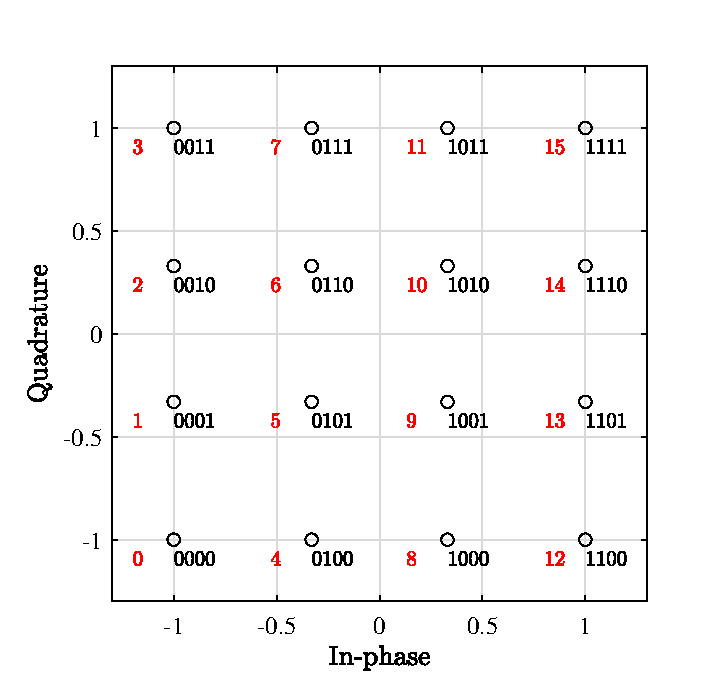
\includegraphics[width=.8\linewidth]{figures/qam16_con.eps}
%     \caption{Ánh xạ các nhóm $4$ bít thành các ký hiệu sử dụng điều chế $16$-QAM.}
%     \label{fig:mapping}
% \end{figure}

% Ma trận kênh truyền $\mathbf{H}$ lấy theo mô hình kênh CBSM i.i.d Rayleigh đã trình bày trong chương~\ref{sec:back}, trong đó, các hệ số phức của kênh truyền được gieo ngẫu nhiên độc lập và cùng phân bố Gauss với giá trị trung bình $\mu$ và phương sai $\sigma^2$ như trên hình~\ref{fig:ray_H}.
% \begin{equation}
% \Re(h_{l, t})=f(x \mid \mu, \sigma)=\frac{1}{\sigma \sqrt{2 \pi}} e^{\frac{-(x-\mu)^2}{2 \sigma^2}}, \quad \text { với } x \in \mathbb{R}
% \end{equation}
% \begin{figure}
%     \centering
%     \begin{subfigure}{.48\linewidth}
%         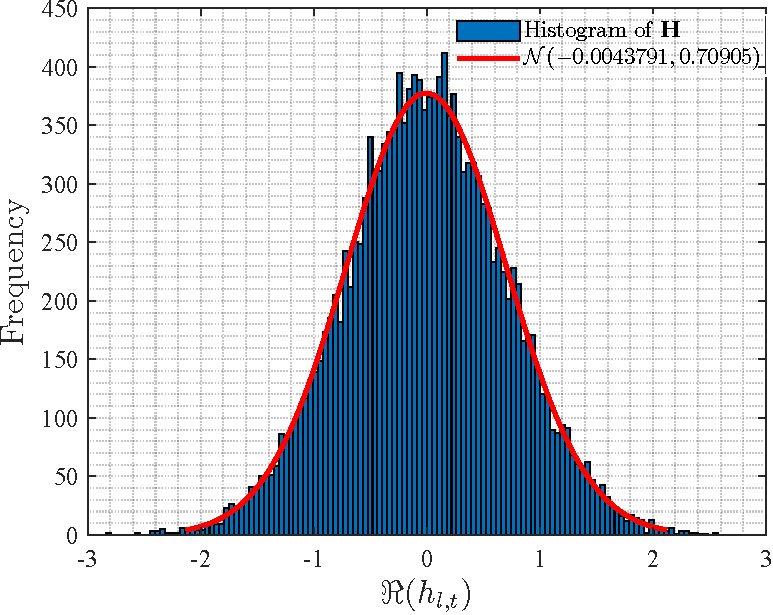
\includegraphics[width=\linewidth]{figures/H.pdf}
%         \caption{$\mathbf{H}$}
%         \label{fig:ray_H}
%     \end{subfigure}
%     \hfill
%     \begin{subfigure}{.48\linewidth}
%         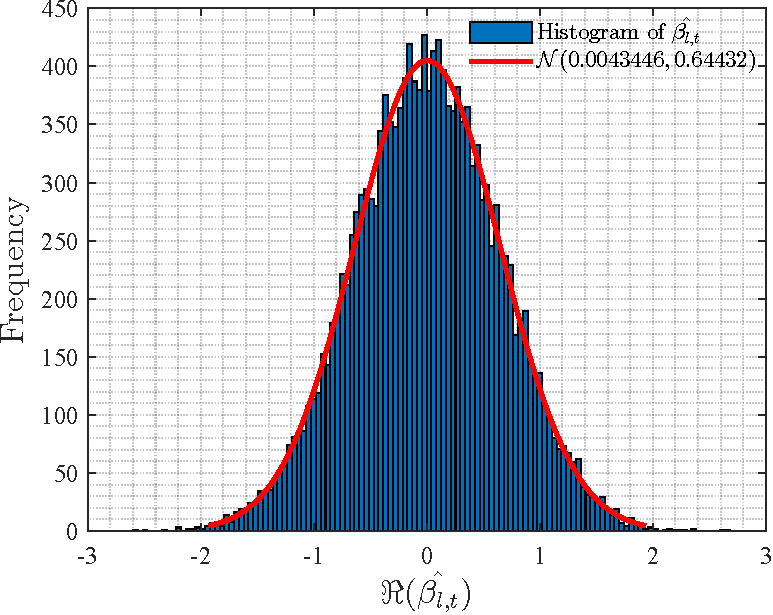
\includegraphics[width=\linewidth]{figures/Beta.pdf}
%         \caption{$\hat{\boldsymbol{\beta}}$}
%         \label{fig:ray_Beta}
%     \end{subfigure}
%     \caption{Phân bố khi gieo ngẫu nhiên của các hệ số phần thực của $h_{l, t}$ và $ \hat{\beta}_{l, t}$ trong hai ma trận $\mathbf{H}$, $\hat{\boldsymbol{\beta}}$.}
%     \label{fig:ray}
% \end{figure}

% Trong mô hình kênh truyền có cấu trúc, vẫn giữ nguyên cách gieo ngẫu nhiên như ma trận $\mathbf{H}$ như mô hình không sử dụng cấu trúc. Sau đó, từ các thông tin bên lề là DoA và cấu hình mảng ăng-ten thu, các giá trị thuộc ma trận $\hat{\boldsymbol{\beta}}$ được tính ngược lại theo công thức~(\ref{eq:betahat}). Trên hình~\ref{fig:ray_Beta} là biểu diễn histogram các giá trị phần thực $\hat{\beta}_{l, t}$ thuộc ma trận $\hat{\boldsymbol{\beta}}$. Có thể nhận thấy các phần tử trong ma trận $\mathbf{H}$ và $\hat{\boldsymbol{\beta}}$ cùng có phân bố chuẩn với kỳ vọng xấp xỉ bằng $0$. Sự khác nhau nằm ở phương sai của các phân bố này, lần lượt là $\approx \mathcal{N} (0; \frac{1}{\sqrt{2}})$, $\mathcal{N} (0; 0,644)$ ứng với $\Re(h_{l, t})$ và $\Re(\hat{\beta}_{l, t})$. Với phương sai nhỏ hơn, có thể dự đoán rằng các mạng học sâu như ISDNN có cấu trúc có thể cho ra các hệ số của ma trận $\hat{\boldsymbol{\beta}}$ nhanh và chính xác hơn không sử dụng cấu trúc $\mathbf{H}$.
% . Sự khác nhau nằm ở cách sắp xếp các giá trị ngẫu nhiên này để tạo thành hai ma trận kể trên, điều này sẽ dẫn đến các kết quả học khác nhau trong quá trình đào tạo.

% Ngoài việc đào tạo dựa trên các thông tin kênh truyền $\mathbf{H}$ và $\hat{\boldsymbol{\beta}}$ chính xác. Trước hết, xem xét việc đào tạo ISDNN cho mô hình kênh không sử dụng cấu trúc trong trường hợp thông tin $\mathbf{H}$ không chính xác (im - imperfect) để kiểm tra khả năng chịu lỗi của kiến trúc mạng nơ-rơn sâu ISDNN đề xuất. Lý do là trong các điều kiện thực tế, các ma trận đầu vào để đào tạo được đo lường không thể có được sự chính xác hoàn hảo. Hai mức sai số sẽ được xem xét đó là $1\%$ và $5\%$.
% \begin{equation}
% \begin{aligned}
%      \mathbf{H}_{im} &= \mathbf{H} \pm 0,01\mathbf{H} \\
%      \mathbf{H}_{im} &= \mathbf{H} \pm 0,05\mathbf{H}
% \end{aligned}
% \end{equation}
% Tương tự, xem xét việc đào tạo kiến trúc mạng ISDNN cho mô hình kênh có cấu trúc trong trường hợp cả thông tin $\mathbf{H}$ và ${\boldsymbol{\varphi}}$ đều có sai số. Sai số từ $\mathbf{H}$ vẫn tương tự như giả thiết của mô hình kênh không sử dụng cấu trúc. Sai số của dữ liệu đầu vào ${\boldsymbol{\varphi}}$ đến từ việc ước lượng sai các giá trị $(\boldsymbol{\theta}, \boldsymbol{\phi})$. Tương tự như trên, hai mức sai số của ${\boldsymbol{\varphi}}$ sẽ được xem xét đó là $1\%$ và $5\%$. Sai số của ${\boldsymbol{\varphi}}$ được gọi là ``\textbf{sai số của thông tin bên lề}''.
% \begin{equation}
%     \begin{aligned}
%          {\boldsymbol{\varphi}}_{im} &= {\boldsymbol{\varphi}} \pm 0,01{\boldsymbol{\varphi}} \\
%          {\boldsymbol{\varphi}}_{im} &= {\boldsymbol{\varphi}} \pm 0,05{\boldsymbol{\varphi}}
%     \end{aligned}
% \end{equation}

Sau khi đi qua kênh truyền $\mathbf{H}$, các ký hiệu sẽ được cộng thêm với AWGN ở các giá trị $\operatorname{SNR}$ khác nhau tính theo thang dB (decibel). 
\begin{equation}
\operatorname{SNR} = 10 \log \left(\frac{\mathbb{E}\left(\|\mathbf{H s}\|_2^2\right)}{\mathbb{E}\left(\|\mathbf{w}\|_2^2\right)}\right)~\text{(dB)}
\end{equation}
Cụ thể, trong bộ dữ liệu đào tạo, $5$ ngưỡng $\operatorname{SNR}$ khác nhau, lần lượt là $0, 5, 10, 15,$ và~$20$~dB được thêm vào các mẫu huấn luyện, sau đó bộ dữ liệu này được trộn ngẫu nhiên.

\subsection{Đào tạo và đánh giá kiến trúc mạng nơ-ron sâu đề xuất}

\subsubsection*{\textbf{Phương pháp đánh giá}}

% Sau khi đã tạo được các bộ dữ liệu, việc đào tạo được triển khai trên máy tính với cấu hình: vi xử lý Intel Core i9-10900, 64~GB RAM. Ngôn ngữ lập trình Python được lựa chọn để xây dựng các mô phỏng của ISDNN và DetNet. 
Thư viện nền tảng Pytorch được sử dụng cho ISDNN, và Tensorflow cho DetNet. Mã nguồn của DetNet lấy từ kho lưu trữ công khai của nhóm tác giả trên bài báo gốc tại Github\footnote{\url{https://github.com/neevsamuel/DeepMIMODetection}}. Sai số của các mạng nơ-ron này được đánh giá thông qua thông số BER tương ứng là số bít ước lượng sai ($N_e$) chia cho tổng số bít. Ở bước thử nghiệm, $100$ bộ dữ liệu thử nghiệm, mỗi bộ gồm $5.000$ mẫu được tạo ra, kết quả ước lượng của các mô hình thu được sau quá trình đào tạo được tính bằng BER trung bình của $100$ lần thử nghiệm.
\begin{equation}
    \operatorname{BER} = \frac{1}{100} \sum_{K=1}^{100} \frac{N_e}{5000}
\end{equation}

\subsubsection*{\textbf{So sánh độ phức tạp của các phương pháp}}
Độ phức tạp của các thuật toán sẽ được so sánh như trên bảng~\ref{tab:computational}. Trong đó, hai bộ nhận dạng truyền thống ZF và MMSE đều có độ phức tạp $\mathcal{O}(TL^3)$ do phép nghịch đảo của ma trận $\mathbf{H}$ với kích thước đầy đủ. Tiếp đến, kiến trúc mạng DetNet cho độ phức tạp $\mathcal{O}(TL^2)$ do không phải nghịch đảo ma trận $\mathbf{G}_\mathbf{H}$ nên thành phần phức tạp nhất trong DetNet là các phép nhân ma trận $\mathbf{H}^\top \mathbf{H}$ và $\mathbf{H}^\top \mathbf{H} \hat{\mathbf{s}}_k$. Cuối cùng là độ phức tạp của kiến trúc mạng ISDNN được đề xuất cho cả hai mô hình kênh truyền có cấu trúc và không sử dụng cấu trúc cũng ở mức $\mathcal{O}(TL^2)$. Dù có phép nghịch đảo ma trận $\mathbf{D}^{-1}$ ở đầu vào, tuy nhiên như đã trình bày ở trên, ma trận $\mathbf{D}$ chỉ gồm các phần tử trên đường chéo chính của ma trận Gram. Do vậy, việc nghịch đảo ma trận này chỉ có độ phức tạp $\mathcal{O}(TL)$, vì chỉ cần sử dụng phép biến đổi tuyến tính. Vậy nên, độ phức tạp tổng thể của ISDNN vẫn tương tự như DetNet chỉ dừng ở các phép nhân ma trận. Có thể kết luận rằng, các phương pháp sử dụng học sâu đã giảm thiểu độ phức tạp đi $\mathcal{O}(L)$ so với các bộ ước lượng tuyến tính truyền thống. Đây là khoảng cách rất lớn, vì trong các hệ mMIMO, giá trị của $L$ có thể lên đến hàng nghìn. So sánh riêng hai kiến trúc mạng DNN là DetNet và ISDNN, dù có chung độ phức tạp nhưng nhận thấy số lượng giá trị học của ISDNN là không đáng kể khi so sánh với DetNet. Điều này có được là do các bộ biến đổi tuyến tính ($\mathbf{W}, \mathbf{b}$) trong DetNet ở dưới dạng ma trận và véc-tơ có kích thước lớn. Trong khi đó, ISDNN chỉ yêu cầu hai tham số học vô hướng ($w, b$) cho mỗi bộ biến đổi tại mỗi lớp mạng. Do vậy, chỉ $24$ tham số học cần được sử dụng trong ISDNN, dẫn đến mô hình thu được sau quá trình đào tạo chỉ có kích thước $7$~KB so với $1,236$~KB của DetNet với cùng số lớp mạng là $4$. Đây là lợi thế rất lớn, khi kích thước nhỏ và độ phức tạp thấp giúp làm tăng khả năng ứng dụng trên cả các thiết bị có giá thành thấp.
\begin{table}[t]
    \centering
    \caption{So sánh độ phức tạp của các thuật toán nhận dạng kênh truyền.}
    \label{tab:computational}
    \begin{tabular}{l|c|c}
    \hline
    \hline
    \multicolumn{1}{c|}{\textbf{Bộ nhận dạng}} & \textbf{Độ phức tạp} & \textbf{Số giá trị học} \\ \hline
    ZF & $\mathcal{O}$ ($TL^3$) &  \\ \hline
    MMSE & $\mathcal{O}$ ($TL^3$) &  \\ \hline
    DetNet: 4 layers & $\mathcal{O}$ ($TL^2$) & 105.416 \\ \hline
    ISDNN unstructured& $\mathcal{O}$ ($TL^2$) & 24 \\ \hline
    ISDNN structured& $\mathcal{O}$ ($TL^2$) & 24 \\ \hline
    \end{tabular}
\end{table}

\subsubsection*{\textbf{So sánh độ chính xác của mạng nơ-ron sâu đề xuất với các phương pháp khác}}
% Trên hình~\ref{fig:training_1} là quá trình đào tạo của hai mạng nơ-ron sâu ISDNN và DetNet với số lớp mạng, mô hình kênh khác nhau. Hình~\ref{fig:loss_1} xem xét về thời gian hội tụ thông qua đầu ra của hàm mất mát giữa véc-tơ ký hiệu gốc $\mathbf{s}$ và véc-tơ ký hiệu ước lượng $\mathbf{\hat{s}}$. Nhận thấy, thời gian hội tụ của mạng DetNet với $4$ lớp mạng có phần nhanh hơn so với ISDNN có cấu trúc và không sử dụng cấu trúc cùng số lớp mạng. Tuy nhiên, xét về tổng thể, đầu ra hàm mất mát của ISDNN cả có cấu trúc và không sử dụng cấu trúc cho kết quả tốt hơn so với DetNet cùng số lớp mạng dù phải cần đến vòng đào tạo thứ $12.000$. Xét riêng hai mô hình có cấu trúc và không sử dụng cấu trúc của ISDNN, tốc độ hội tụ và giá trị của hàm mất mát tại vòng lặp cuối cùng khá tương đồng nhau khoảng $4 * 10^{-3}$. Nếu tăng số lớp mạng của DetNet lên $10$, do số lượng tham số học tăng lên đáng kể, thời gian hội tụ và đầu ra mất mát cuối cùng cũng cho kết quả tốt hơn ISDNN chỉ $4$ lớp mạng. Tuy nhiên, đánh đổi ở đây là số lượng tham số học sẽ lên đến $316.244$. Xét về sự hội tụ dựa trên tỷ lệ sai số bít của các kiến trúc như trên hình~\ref{fig:ber_1}. Trước hết, BER của ISDNN chỉ với $4$ lớp mạng sau $20.000$ vòng đào tạo là vượt trội so với DetNet dù $4$ hay $10$ lớp mạng, hội tụ ở giá trị $\operatorname{BER}\approx 4 * 10^{-4}$ và $6*10^{-4}$ lần lượt với mô hình có cấu trúc và không sử dụng cấu trúc. So sánh với DetNet dù với $10$ lớp mạng và lượng tham số học khổng lồ cũng chỉ có đạt được sai số chưa đến $10^{-3}$. Tuy nhiên, từ mô phỏng cũng cho thấy rằng, độ chính xác của DetNet cho thời gian hội tụ là nhanh hơn nhiều so với ISDNN khi chỉ cần đến khoảng $5.000$ vòng đào tạo. Trong quá trình đào tạo, thông qua cả hai thông số BER và hàm mất mát, có thể rút ra nhận xét rằng, kiến trúc ISDNN có cấu trúc cho độ chính xác trong quá trình học là tốt hơn ISDNN không sử dụng cấu trúc và DetNet, tuy nhiên, DetNet lại là mạng có thời gian hội tụ nhanh nhất.
% Với ISDNN có cấu trúc, thời gian đạt đến $\operatorname{BER}\approx 10^{-3}$ là nhanh nhất trong cả $4$ mô hình được xem xét chỉ chưa đến $5.000$ vòng đào tạo. Tuy nhiên sau đó, tương tự như hàm mất mát, giá trị BER của ISDNN có cấu trúc thay đổi liên tục trong khoảng $[10^{-2} \;\; 10^{-3}]$ không theo quy luật nào. Điều này có thể là do hai nguyên nhân: (i), số lượng tham số học của mạng nhỏ, không đủ để học ra giá trị tối ưu ứng với toàn bộ tập dữ liệu huấn luyện; (ii), tập đầu vào $\hat{\mathbf{x}}$ ước lượng được có sai số.

% \begin{figure}[t]
%      \centering
%      \begin{subfigure}[b]{0.48\textwidth}
%          \centering
%          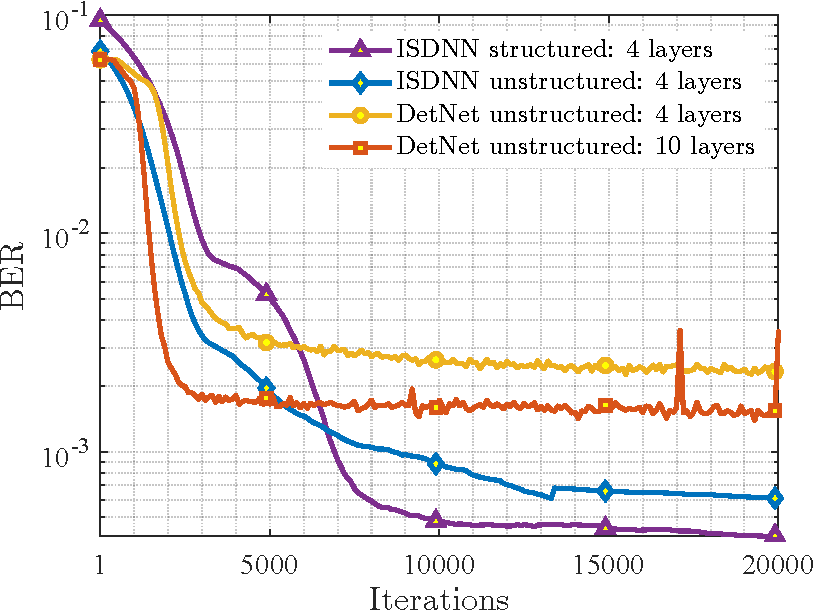
\includegraphics[width=\textwidth]{figures/BER_1.pdf}
%          \caption{BER}
%          \label{fig:ber_1}
%      \end{subfigure}
%      \hfill
%      \begin{subfigure}[b]{0.48\textwidth}
%          \centering
%          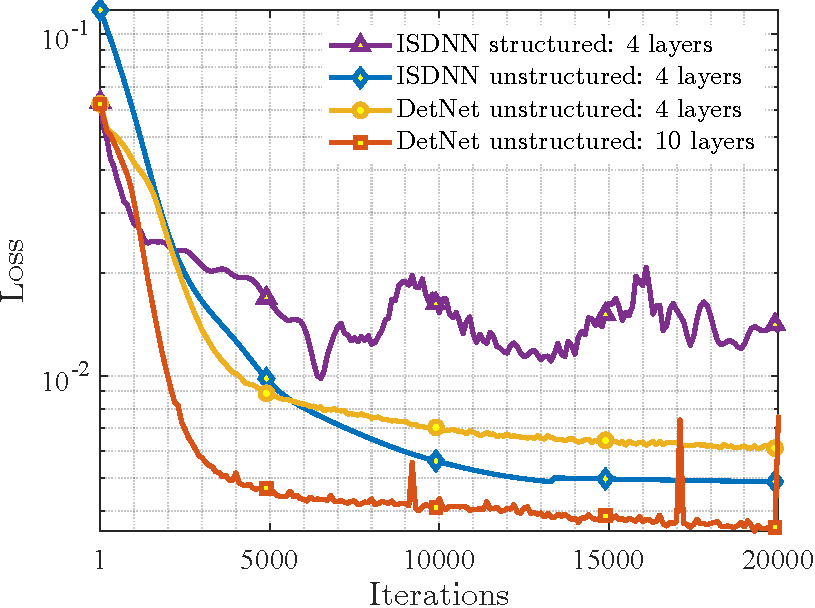
\includegraphics[width=\textwidth]{figures/Loss_1.pdf}
%          \caption{Mất mát}
%          \label{fig:loss_1}
%      \end{subfigure}
%      \hfill
%         \caption{Sự hội tụ của quá trình đào tạo mạng ISDNN và DetNet.}
%         \label{fig:training_1}
% \end{figure}
\begin{figure}[t]
    \centering
    \begin{subfigure}{\linewidth}
        \centering
        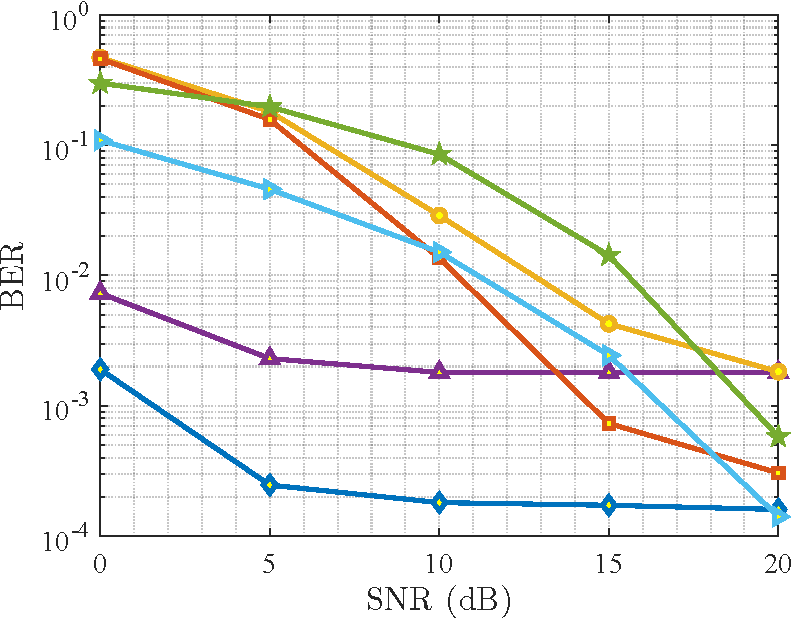
\includegraphics[width=.6\linewidth]{figures/performance_1.pdf}
    \end{subfigure}
    \hfill
    \begin{subfigure}{\linewidth}
        \centering
        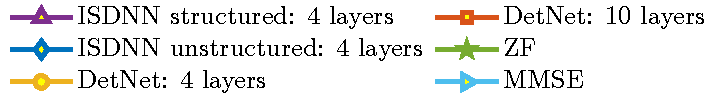
\includegraphics[width=.5\linewidth]{figures/lg_performance_1.pdf}
    \end{subfigure}
    \caption{Độ chính xác của mạng ISDNN so sánh với DetNet và các bộ nhận dạng tuyến tính.}
    \label{fig:isdnn}
\end{figure}

% Sau quá trình đào tạo, kiểm tra mô hình thu được trên các bộ dữ liệu thử nghiệm độc lập với tập dữ liệu huấn luyện. 
Kết quả thu được khi so sánh độ chính xác của các phương pháp nhận dạng kênh truyền gồm ZF, MMSE, DetNet, và ISDNN khi SNR thay đổi được biểu diễn trên hình~\ref{fig:isdnn}. 
% Trước hết, có thể kết luận, độ chính xác của mạng ISDNN đề xuất là vượt trội so với các phương pháp còn lại. Khi so sánh với hai phương pháp tuyến tính là ZF và MMSE, đường BER của ISDNN và DetNet đều cho thấy sự khác biệt, khi độ dốc của BER từ các mạng DNN giảm dần theo SNR còn ZF và MMSE thì ngược lại. Phải cần đến mức $\operatorname{SNR}=20$~dB, phương pháp MMSE mới đạt đến độ chính xác của ISDNN không sử dụng cấu trúc tức $\operatorname{BER}\approx 1,5* 10^{-4}$, do giải thuật gốc ISD cũng xuất phát từ MMSE nên có thể coi đây là giá trị tối ưu của ISD. Khi so sánh với mạng nơ-ron sâu DetNet gồm $4$ lớp mạng, ISDNN không sử dụng cấu trúc cho độ lợi về BER đạt $10^2$ tại các mức SNR thấp, và $10^1$ tại SNR cao. ISDNN có cấu trúc cho tỷ lệ sai số bít thấp hơn mạng không sử dụng cấu trúc, tuy nhiên độ lợi là chưa thực sự vượt trội, ở $\operatorname{SNR}=20$~dB, tỷ lệ lỗi bít đạt $\approx 10^{-4}$. Khi tăng số lớp của DetNet lên $10$, cũng tương tự như quá trình huấn luyện, độ chính xác đã được cải thiện, tuy nhiên dù SNR ở mức cao như $20$~dB, BER của DetNet cũng chỉ tiệm cận được đến độ chính xác của ISDNN không sử dụng cấu trúc với $4$ lớp mạng.
Có thể rút ra nhận xét, kiến trúc ISDNN ngoài việc cho độ chính xác vượt trội so với ZF, MMSE, và DetNet còn có ưu điểm là BER không có sự biến đổi quá lớn ở các mức SNR khác nhau. Đây là ưu điểm quan trọng của việc sử dụng DNN cho việc nhận dạng kênh truyền, khi tạp âm/công suất phát luôn là một vấn đề mà các thế hệ mạng viễn thông thế hệ mới như 5G quan tâm. Nếu độ chính xác của việc nhận dạng không bị phụ thuộc nhiều vào SNR thì mật độ bao phủ, cũng như hiệu quả về năng lượng là những lợi ích có thể khai thác.

\subsubsection*{\textbf{Xem xét độ chính xác của mạng nơ-ron sâu ISDNN khi có sai số trong tập dữ liệu đào tạo}}
% Tiếp theo, xem xét đến tính chống chịu lỗi của mạng nơ-ron sâu ISDNN. Như đã trình bày ở trên, để có thể được áp dụng thực tế, các bộ dữ liệu cần được thu thập từ các hệ thống viễn thông thực. Tuy nhiên, sai số khi đo lường các đầu vào cho việc đào tạo là không thể tránh khỏi. 
Trong phần này: (i), ma trận kênh truyền $\mathbf{H}$ được giả sử là có sự sai khác $1$\% và $5$\% so với $\mathbf{H}$ hoàn hảo; (ii), cả ma trận kênh truyền $\mathbf{H}$ và ma trận thông tin bên lề ${\boldsymbol{\varphi}}$ đều có sai số là $1$\% và $5$\% so với giá trị thực tế. 
% \begin{figure}[ht]
%     \centering
%     \begin{subfigure}[b]{0.48\textwidth}
%         \centering
%         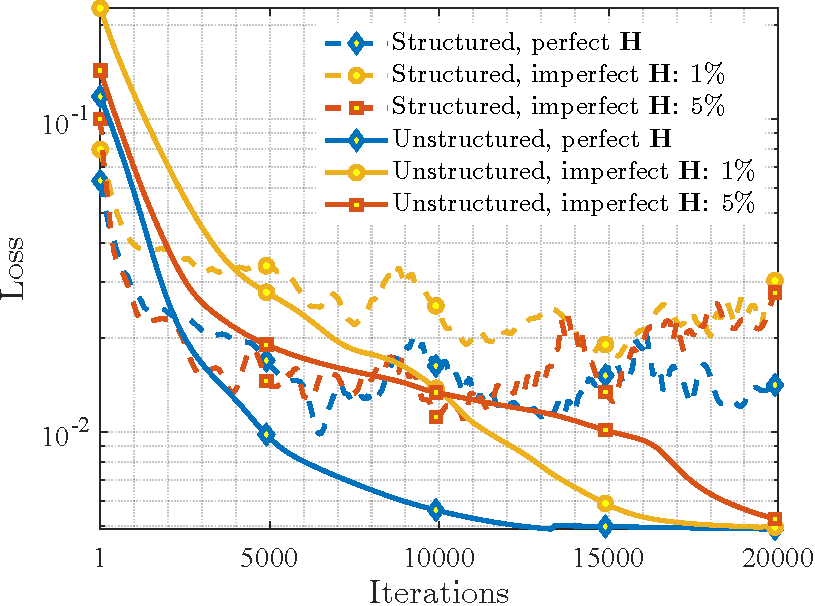
\includegraphics[width=\textwidth]{figures/BER_2.pdf}
%         \caption{BER}
%         \label{fig:ber_2}
%     \end{subfigure}
%     \hfill
%     \begin{subfigure}[b]{0.48\textwidth}
%         \centering
%         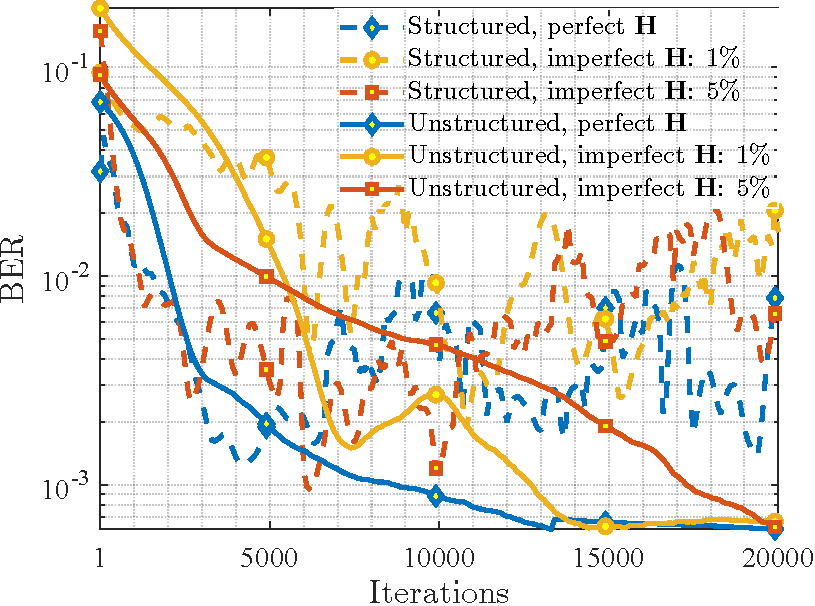
\includegraphics[width=\textwidth]{figures/Loss_2.pdf}
%         \caption{Mất mát}
%         \label{fig:loss_2}
%     \end{subfigure}
%     \hfill
%     \begin{subfigure}{\linewidth}
%         \centering
%         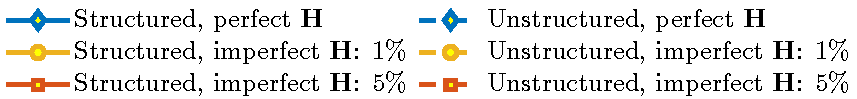
\includegraphics[width=.8\linewidth]{figures/lg_performance_21.pdf}
%     \end{subfigure}
%     \caption{Sự hội tụ của quá trình đào tạo các mạng ISDNN với các sai số kênh truyền đầu vào khác nhau.}
%     \label{fig:training_2}
% \end{figure}

% Trên hình~\ref{fig:training_2} là kết quả của việc đào tạo mạng ISDNN có cấu trúc và không sử dụng cấu trúc với $3$ bộ dữ liệu có các mức sai số kênh truyền khác nhau. Đầu tiên, hình~\ref{fig:loss_2} cho thấy rõ ràng sai số của dữ liệu đầu vào ảnh hưởng trực tiếp đến sự hội tụ của một mạng DNN. 
% Cả hai kiến trúc ISDNN với kênh truyền chính xác cho tốc độ hội tụ về hàm mất mát là nhanh hơn đáng kể khi so với trường hợp kênh truyền có sai số. Với sai số $1$\% cần đến $14.000$ và $18.000$ vòng đào tạo lần lượt với mạng có cấu trúc và không sử dụng cấu trúc để đầu ra của hàm mất mát hội tụ. Tương tự, khi sai số là $5$\%, sau $20.000$ vòng đào tạo vẫn chưa có được sự hội tụ của hàm mất mát. Tuy có sự khác nhau về tốc độ, nhưng giá trị cuối cùng của hàm mất mát tại cả $6$ trường hợp đều khá tương đồng khoảng $5*10^{-3}$.
% Tiếp theo, về độ chính xác trong quá trình đào tạo cũng cho kết quả tương đồng, biểu diễn trên hình~\ref{fig:ber_2}. Khi dữ liệu kênh truyền có sai số, đường BER trong quá trình học của các mạng ISDNN có sự không ổn định và cần đến thêm ít nhất $5.000$ vòng đào tạo để đạt được giá trị hội tụ. 
% Do đó, xét cả hàm mất mát và BER, kiến trúc ISDNN vẫn có thể thích nghi với sai số $1$\% của ma trận kênh truyền dù ảnh hưởng đến thời gian huấn luyện cần để hội tụ nhưng vẫn sẽ hội tụ ở giá trị khá tương đương với kênh truyền hoàn hảo. 
\begin{figure}[H]
    \centering
    \begin{subfigure}{\linewidth}
        \centering
        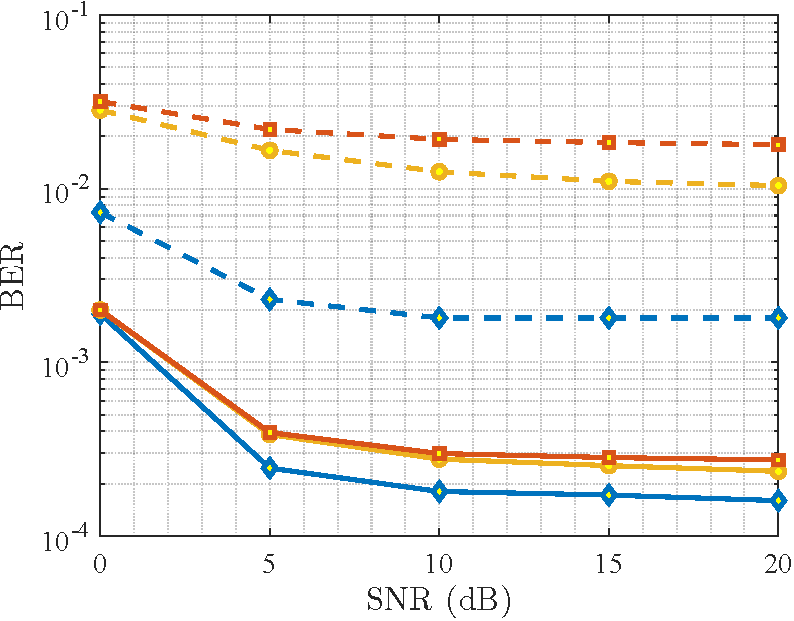
\includegraphics[width=.6\linewidth]{figures/performance_2.pdf}
    \end{subfigure}
    \hfill
    \begin{subfigure}{\linewidth}
        \centering
        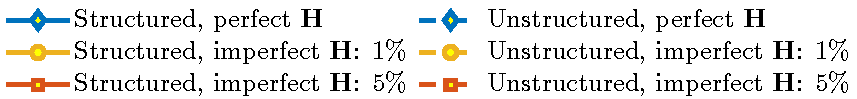
\includegraphics[width=.6\linewidth]{figures/lg_performance_21.pdf}
    \end{subfigure}
    \caption{Độ chính xác của mạng ISDNN với các sai số kênh truyền đầu vào khác nhau.}
    \label{fig:isdnn_1}
\end{figure}

Mô hình thu được sau quá trình đào tạo ở cả ba trường hợp sẽ được đánh giá trên các bộ dữ liệu thử nghiệm, kết quả thu được như trên hình~\ref{fig:isdnn_1}. Dễ nhận thấy, sự tương quan của sai số ma trận kênh truyền đầu vào với BER đầu ra của mô hình đã huấn luyện. Với ISDNN không sử dụng cấu trúc, ở các giá trị $\operatorname{SNR}\ge 5$~dB, BER trong trường hợp kênh truyền chính xác và có sai số khá ổn định, lần lượt ở mức~$\approx 1,7 * 10^{-4}$, $2,5* 10^{-4}$, và $2,8* 10^{-4}$. 
Điều tương tự với ISDNN có cấu trúc khi BER tỷ lệ nghịch với sai số của tập dữ liệu đầu vào. Khi $\operatorname{SNR}\ge 5$~dB, các giá trị BER trung bình lần lượt của ISDNN có cấu trúc là~$\approx 1,1 * 10^{-4}$, $1,3* 10^{-4}$, và $1,7* 10^{-4}$. 
% Nếu so sánh mức sai số này với các kết quả thu được trên hình~\ref{fig:isdnn}, kể cả ở mức sai số $5$\% của ma trận kênh truyền, ISDNN không sử dụng cấu trúc vẫn cho sai số tương đương với DetNet $10$ lớp mạng và vượt trội DetNet nếu chỉ $4$ lớp mạng. Khi so sánh với hai bộ ước lượng tuyến tính, MMSE (ISD gốc) sẽ tốt hơn ISDNN không sử dụng cấu trúc với sai số dữ liệu $5$\% nếu SNR ở các giá trị $\ge 15$~dB. Ngược lại, nếu sử dụng ZF hoặc SNR thấp hơn thì ISDNN vẫn cho sai số tốt hơn. 
Từ các kết quả trên, có thể thấy sự ảnh hưởng của dữ liệu đầu vào tới ISDNN nói riêng và các mạng DNN nói chung, tuy nhiên ở các mức sai số nhỏ, mô hình đầu ra vẫn sẽ cho độ chính xác ở mức chấp nhận được, và vẫn sẽ hơn các giải thuật tuyến tính hay mạng DetNet.
% Đây chính là tiềm năng để triển khai ISDNN với các bộ dữ liệu thực và trên các hệ thống viễn thông thực tế trong tương lai.
% \begin{figure}[ht]
%      \centering
%      \begin{subfigure}[b]{0.48\textwidth}
%          \centering
%          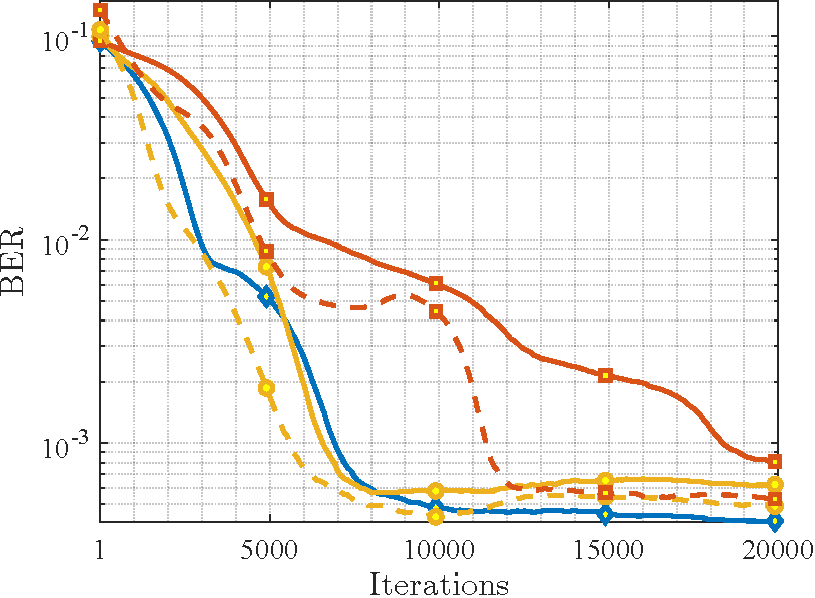
\includegraphics[width=\textwidth]{figures/BER_3.pdf}
%          \caption{BER}
%          \label{fig:ber_3}
%      \end{subfigure}
%      \hfill
%      \begin{subfigure}[b]{0.48\textwidth}
%          \centering
%          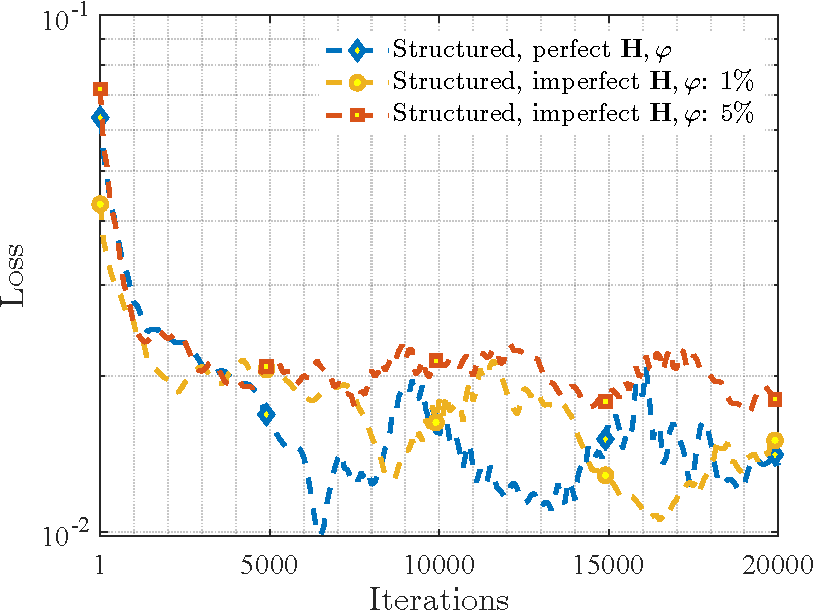
\includegraphics[width=\textwidth]{figures/Loss_3.pdf}
%          \caption{Mất mát}
%          \label{fig:loss_3}
%      \end{subfigure}
%      \hfill
%     \begin{subfigure}{\linewidth}
%         \centering
%         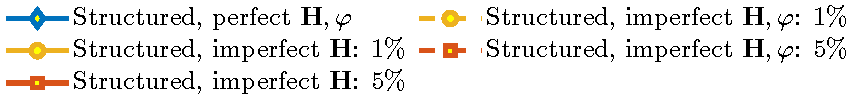
\includegraphics[width=.8\linewidth]{figures/lg_performance_31.pdf}
%     \end{subfigure}
%     \caption{Sự hội tụ của quá trình đào tạo các mạng ISDNN có cấu trúc với các sai số kênh truyền và thông tin bên lề đầu vào khác nhau.}
%     \label{fig:training_3}
% \end{figure}

% Trên hình~\ref{fig:training_3} là kết quả đào tạo của mạng ISDNN có cấu trúc khi các bộ dữ liệu huấn luyện có cả sai số trong $\mathbf{H}$ và ${\boldsymbol{\varphi}}$. Với việc cả hai ma trận trên đều có sai số sẽ hình thành sai số tích lũy cho các đầu vào như $\hat{\mathbf{s}}, \hat{\mathbf{x}}, \mathbf{D},~\ldots$ có thể gây khó khăn cho bộ nhận dạng. Trước hết trên hình~\ref{fig:loss_3} là đầu ra của hàm mất mát thu được trong suốt quá trình đào tạo. Tuy có thêm sai số đầu vào từ DoA, nhưng giá trị đầu ra của hàm mất mát lại cho thấy điều ngược lại, khi có thêm sai số này, mạng ISDNN hội tụ nhanh hơn cả trường hợp khi chỉ có sai số của kênh truyền $\mathbf{H}$. Đặc biệt, với trường hợp cả $\mathbf{H}$ và ${\boldsymbol{\varphi}}$ đều có sai số $5\%$, sau $12.000$ vòng đào tạo, giá trị hàm mất mát đã đạt được giá trị hội tụ và ổn định như trường hợp không có sai số. Tương tự với kết quả của BER trong quá trình đào tạo trên hình~\ref{fig:ber_3}, khi có thêm sai số của $\boldsymbol{\varphi}$, đường BER còn có độ lớn hơn trong trường hợp chỉ có sai số của ma trận kênh truyền.
% Chỉ sau $3.000$ vòng đào tạo, cả ba bộ dữ liệu đều cho ra giá trị hàm mất mát khoảng $2*10^{-2}$. Sau đó, trong trường hợp không có sai số và sai số $1$\% trong tập huấn luyện, giá trị của hàm mất mát vẫn tiếp tục đi xuống nhưng vẫn biến thiên, không hội tụ. Trong khi đó, trường hợp sai số $5$\% lại cho ra giá trị khá ổn định xung quanh khoảng $2*10^{-2}$. Với BER trên hình~\ref{fig:ber_3}, cả ba tập dữ liệu đều có thời điểm đạt được $\operatorname{BER} \approx 10^{-3}$ nhưng đều không giữ được giá trị này mà tiếp tục biến thiên không theo quy luật.

% Mạng ISDNN có cấu trúc được lưu tại vòng lặp cuối cùng của việc học và thử nghiệm với các giá trị SNR khác nhau như trên hình. 
Khi có sai số về ma trận $\boldsymbol{\varphi}$, đường BER đầu ra sẽ cho kết quả kém hơn một chút so với khi chỉ có sai số về $\mathbf{H}$ như trên hình~\ref{fig:isdnn_3}. Tuy nhiên, cũng như trong quá trình học, đường BER khi sai số của $\mathbf{H}$ và $\boldsymbol{\varphi}$ ở mức $5\%$ cho kết quả không ổn định. Tại $\operatorname{SNR}=15$~dB, BER của ISDNN còn tốt hơn trường hợp chỉ có sai số $1\%$ của bộ dữ liệu. Nguyên nhân có thể xuất phát từ việc gieo ngẫu nhiên những sai số trong bộ dữ liệu đầu vào, tạo nên ma trận $\hat{\boldsymbol{\beta}}$ tốt hơn ở giá trị SNR này. Trong trong hợp này, so sánh với hình~\ref{fig:isdnn_1}, kết quả mô hình đầu ra trong hai trường hợp có sai số từ $\mathbf{H}$ và thông tin bên lề của mạng ISDNN có cấu trúc là tương đương với mạng ISDNN không sử dụng cấu trúc chỉ có sai số về ma trận kênh truyền.
% \section{Kết luận chương}
\begin{figure}[H]
    \centering
    \begin{subfigure}{\linewidth}
        \centering
        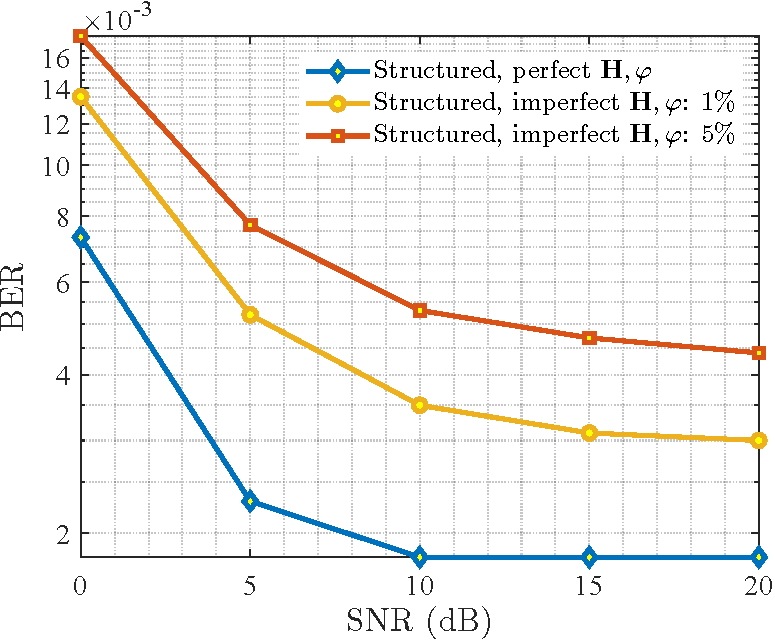
\includegraphics[width=.6\linewidth]{figures/performance_3.pdf}
    \end{subfigure}
    \hfill
    \begin{subfigure}{\linewidth}
        \centering
        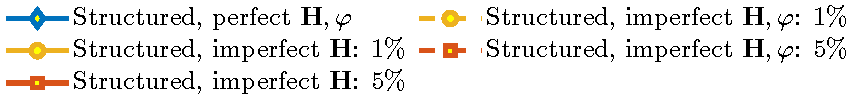
\includegraphics[width=.6\linewidth]{figures/lg_performance_31.pdf}
    \end{subfigure}
    \caption{Độ chính xác của mạng ISDNN có cấu trúc với các sai số kênh truyền và thông tin bên lề đầu vào khác nhau.}
    \label{fig:isdnn_3}
\end{figure}
% Trong chương này, tác giả đã trình bày khái quát về việc sử dụng DNN và mở rộng sâu cho việc nhận dạng kênh truyền. Tiếp đến, một kiến trúc mạng nơ-ron sâu tên DetNet đã được đề xuất trước đây được trình bày ngắn gọn. Từ một phương pháp nhận dạng không mù với độ phức tạp thấp ISD đã được công bố trước đó, kiến trúc ISDNN mới được đề xuất cho cả hai mô hình kênh truyền có cấu trúc và không sử dụng cấu trúc sử dụng phương pháp mở rộng sâu. Kết quả mô phỏng đã chỉ ra hiệu năng về độ chính xác và độ phức tạp của kiến trúc ISDNN được đề xuất. Trước hết, về độ chính xác, ISDNN cho kết quả vượt trội so với các thuật toán nhận dạng tuyến tính không mù như ZF, MMSE, và mạng nơ-ron sâu DetNet dù với số lượng lớp mạng ít hơn. Về độ phức tạp, so với các giải thuật tuyến tính, ISDNN cho độ lợi $\mathcal{O}(L)$ tương tự như DetNet. Hơn nữa, ISDNN chỉ cần $24$ tham số học cho $4$ lớp mạng khi so sánh với $105.416$ tham số của mạng DetNet cùng số lớp mạng. Từ hai khía cạnh trên, kết luận mạng ISDNN đã giải quyết cả hai vấn đề là độ phức tạp, và chính xác đã được đề ra ở phần Mở đầu. Kiến trúc ISDNN được đề xuất cho mô hình kênh truyền có cấu trúc cũng cho độ chính xác là tốt hơn so với ISDNN không sử dụng cấu trúc như đã chỉ ra trong chương~\ref{sec:CRB}.
% Ngoài ra, để xem xét khả năng ứng dụng vào thực tế, hiệu suất của ISDNN được xem xét nếu có sai số trong các bộ dữ liệu đầu vào, có thể xảy ra bởi sai số đo lượng. Các kết quả mô phỏng chỉ ra sự ảnh hưởng của tập dữ liệu huấn luyện đến kết quả đào tạo. Tuy nhiên, sai số cũng ở mức chấp nhận được và vẫn là tốt hơn nếu so sánh với các phương pháp đã kể trên. 